\documentclass[12pt, a4paper]{article}

% ── Packages ───────────────────────────────────────────────
\usepackage[utf8]{inputenc}
\usepackage[T1]{fontenc}
\usepackage{graphicx}
\usepackage{amsmath}
\usepackage{amssymb}
\usepackage{booktabs}
\usepackage{float}
\usepackage{geometry}
\usepackage{setspace}
\usepackage{hyperref}
\usepackage{caption}
\usepackage{subcaption}
\usepackage{xcolor}
\usepackage{enumitem}
\usepackage{titlesec}
\usepackage{fancyhdr}
\usepackage{tabularx}
\usepackage{multirow}
\usepackage{array}
\usepackage{parskip}

\geometry{a4paper, margin=1in}
\onehalfspacing

\newcommand{\rupee}{\textrm{Rs.}\,}

\hypersetup{
    colorlinks=true,
    linkcolor=blue!60!black,
    citecolor=blue!60!black,
    urlcolor=blue!60!black,
}

% ── Header / Footer ───────────────────────────────────────
\pagestyle{fancy}
\fancyhf{}
\fancyhead[L]{\small RDL725 - Field Assignment}
\fancyhead[R]{\small Sunder Nursery}
\fancyfoot[C]{\thepage}
\renewcommand{\headrulewidth}{0.4pt}

% ───────────────────────────────────────────────────────────
\begin{document}

% ════════════════════════════════════════════════════════════
%  TITLE PAGE
% ════════════════════════════════════════════════════════════
\begin{titlepage}
    \centering
    \vspace*{0.5cm}

    % Logo
    
\includegraphics[height=3.5cm]{../Images/iitd_logo.jpeg}

    \vspace{0.8cm}

    {\Large \textbf{Indian Institute of Technology Delhi} \par}
    \vspace{0.2cm}
    {\large Department of Chemical Engineering \par}

    \vspace{0.8cm}

    {\LARGE \bfseries RDL725 - Ecological Perspective \\ of Growth and Development \par}

    \vspace{0.7cm}

    {\Huge \bfseries Field Assignment \par}
    \vspace{0.4cm}
    {\Large \textit{Ecological Evaluation of Sunder Nursery \\ Using the Contingent Valuation Method} \par}

    \vspace{1cm}

    {\large \textbf{Submitted by} \par}
    \vspace{0.3cm}
    \begin{tabular}{ll}
        Prem Bhugra          & 2022CH71038 \\
        Sakhare Yash Balram  & 2022CH71496 \\
        Ninad Narsing Gawade & 2022CH71493 \\
        Nitin Verma          & 2022CH11031 \\
    \end{tabular}

    \vspace{0.8cm}

    \begin{tabular}{ll}
        \textbf{Course Coordinator:} & Prof.\ Vivek Kumar \\
        \textbf{Teaching Assistants:} & Nandita Pawar, Rahul Dwivedi \\
    \end{tabular}

    \vfill
\end{titlepage}

% ════════════════════════════════════════════════════════════
%  TABLE OF CONTENTS
% ════════════════════════════════════════════════════════════
\tableofcontents
\newpage

% ════════════════════════════════════════════════════════════
%  1.  INTRODUCTION
% ════════════════════════════════════════════════════════════
\section{Introduction}

Environmental resources like urban parks and heritage sites provide a wide range of benefits to society-recreational enjoyment, ecological balance, cultural preservation, and aesthetic pleasure. However, because most of these benefits are not traded in any market, they have no ``price tag,'' and their true economic value often goes unrecognized by policy-makers and the public alike.

This report presents an ecological evaluation of \textbf{Sunder Nursery}, a 90-acre heritage park in New Delhi, using the \textbf{Contingent Valuation Method (CVM)}. Our group visited the site on a Friday evening (10 April 2026) and surveyed 45 visitors using a structured bilingual questionnaire. The survey captured visitors' willingness to pay (WTP) for the park's continued conservation, along with travel cost data that enables a complementary analysis using the \textbf{Travel Cost Method (TCM)}.

The objective is to estimate the \textbf{Total Economic Value (TEV)} of Sunder Nursery, which includes both the direct use value enjoyed by current visitors and the non-use values (option, bequest, and existence values) that extend well beyond the park's gates.

% ════════════════════════════════════════════════════════════
%  2.  SITE DESCRIPTION
% ════════════════════════════════════════════════════════════
\section{Site Description and Ecological Background}

\subsection{History and Restoration}

Sunder Nursery is located in the Nizamuddin area of New Delhi, immediately adjacent to Humayun's Tomb-a UNESCO World Heritage Site. The site traces its origins to the 16th century, when it served as a Mughal-era nursery for royal gardens and housed several tombs and garden pavilions.

After Indian independence, the site was reduced to a government plant nursery, and most of its historical structures fell into disrepair. In 2007, the \textbf{Aga Khan Trust for Culture (AKTC)}, in partnership with the Central Public Works Department (CPWD) and the South Delhi Municipal Corporation, launched one of India's largest urban conservation projects to restore the site. After over a decade of work, Sunder Nursery was reopened to the public in \textbf{February 2018} as a fully restored heritage park [6].

\subsection{Ecological Features}

\begin{itemize}[nosep]
    \item \textbf{Area:} 90 acres (approximately 36 hectares)
    \item \textbf{Flora:} Over 300 tree species and 80+ flowering plant varieties spread across themed zones-the arboretum, the ``Garden of Senses,'' native-plant nursery areas, and seasonal flower beds
    \item \textbf{Fauna:} More than 80 bird species have been recorded, including peacocks, parrots, eagles, barbets, mynas, and migratory ducks; butterfly populations are also notable
    \item \textbf{Heritage:} Six restored Mughal-era monuments, including Sundarwala Burj, Sundarwala Mahal, Lakkarwala Burj, and the tomb of Mirza Muzaffar Hussain
    \item \textbf{Water systems:} Restored Mughal-era water channels, lakeside areas, and fountains that support aquatic habitats
\end{itemize}

\begin{figure}[H]
    \centering
    \begin{subfigure}[b]{0.48\textwidth}
        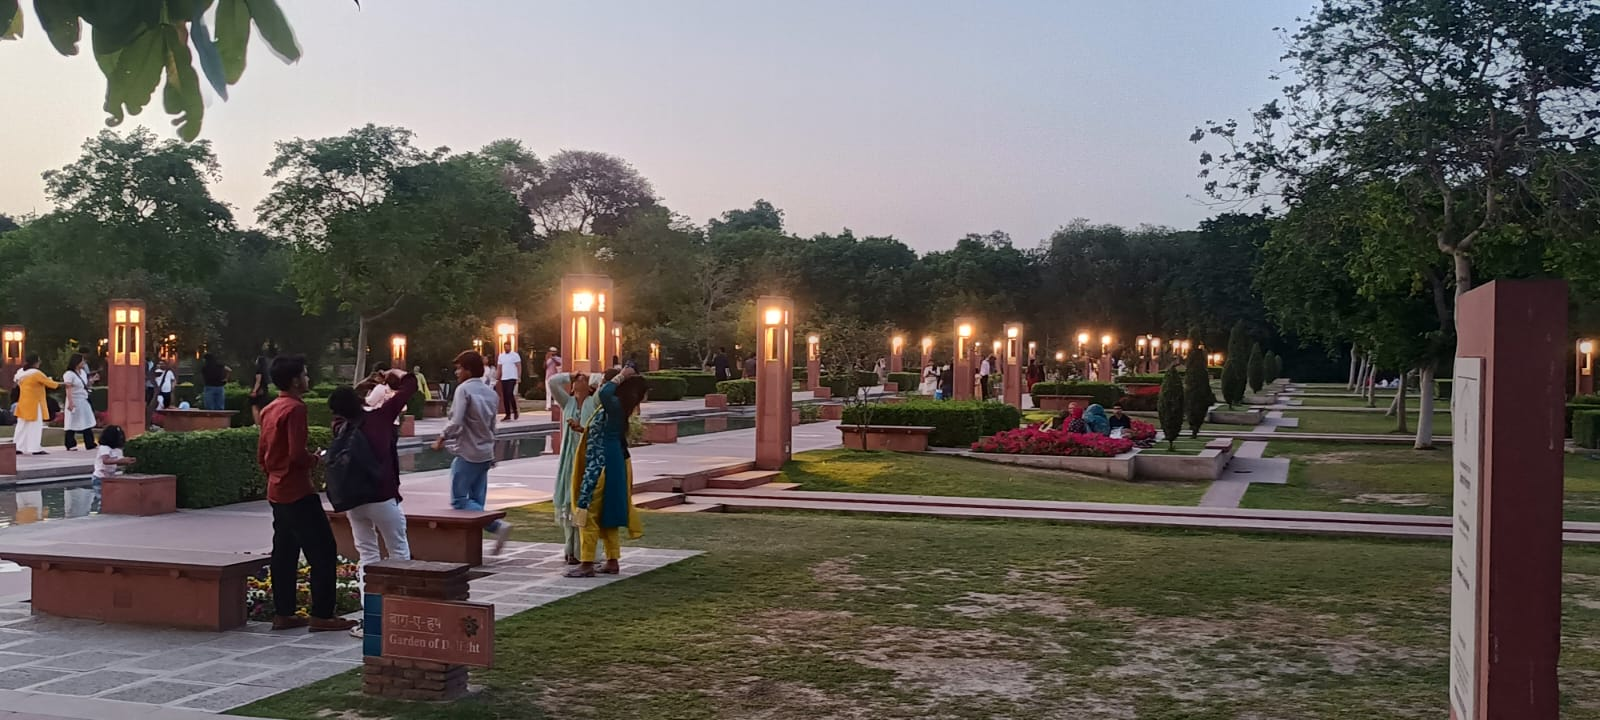
\includegraphics[width=\textwidth, height=6cm, keepaspectratio=false]{../Images/1.jpeg}
        \caption{Garden of Delight at dusk}
    \end{subfigure}
    \hfill
    \begin{subfigure}[b]{0.48\textwidth}
        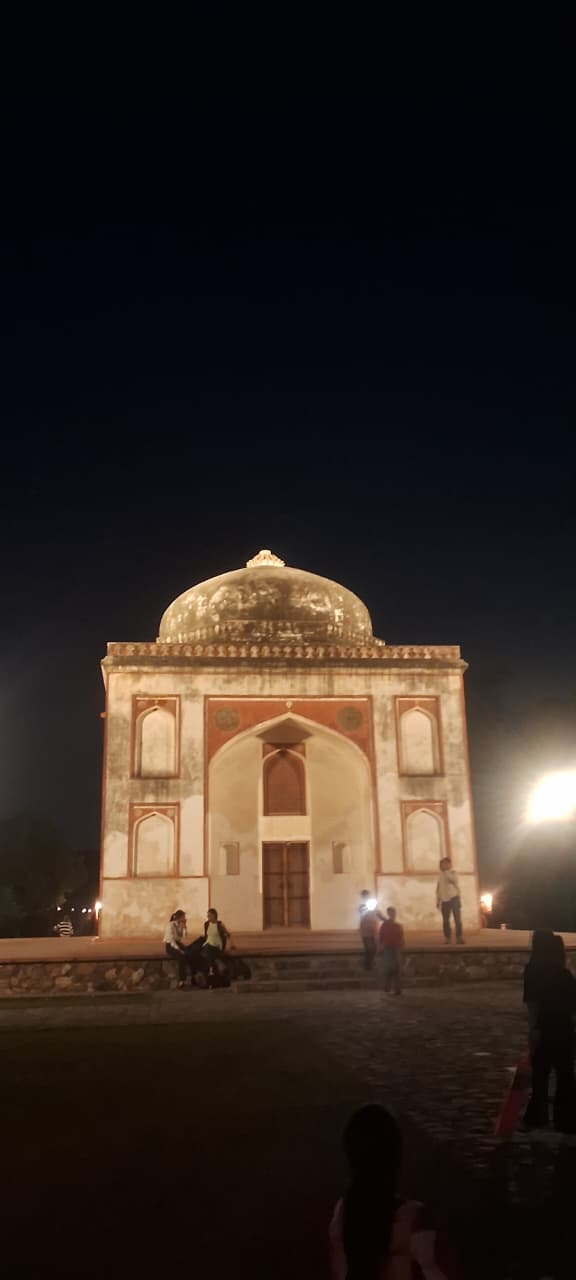
\includegraphics[width=\textwidth, height=6cm, keepaspectratio=false]{../Images/4.jpeg}
        \caption{Sundarwala Burj at night}
    \end{subfigure}
    \caption{Sunder Nursery: heritage and landscape (photographs taken during our field visit).}
    \label{fig:site_overview}
\end{figure}

\subsection{Biodiversity and Green Cover}

The restoration project has turned what was once a neglected compound into a thriving urban ecosystem. The nursery is home to native tree species such as \textit{Azadirachta indica} (Neem), \textit{Ficus religiosa} (Peepal), and \textit{Dalbergia sissoo} (Shisham), alongside ornamental plantings that attract pollinators year-round. The water bodies within the park support aquatic vegetation including lotus and water lilies (Figure~\ref{fig:flora}).

\begin{figure}[H]
    \centering
    \begin{subfigure}[b]{0.32\textwidth}
        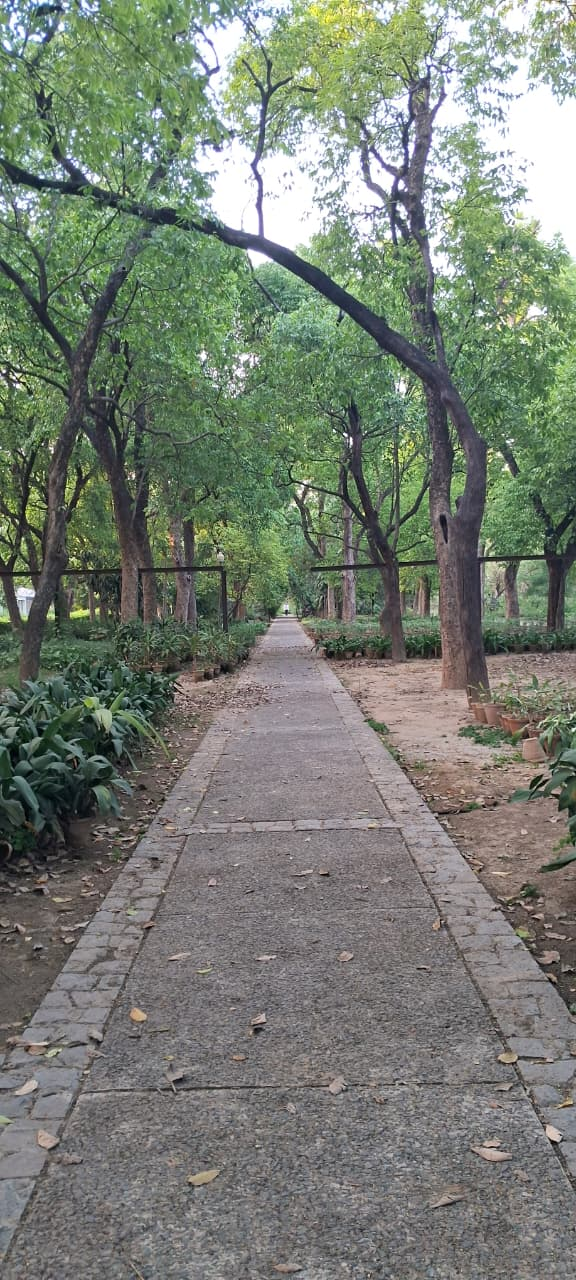
\includegraphics[width=\textwidth, height=5cm, keepaspectratio=false]{../Images/8.jpeg}
        \caption{Tree-lined pathway}
    \end{subfigure}
    \hfill
    \begin{subfigure}[b]{0.32\textwidth}
        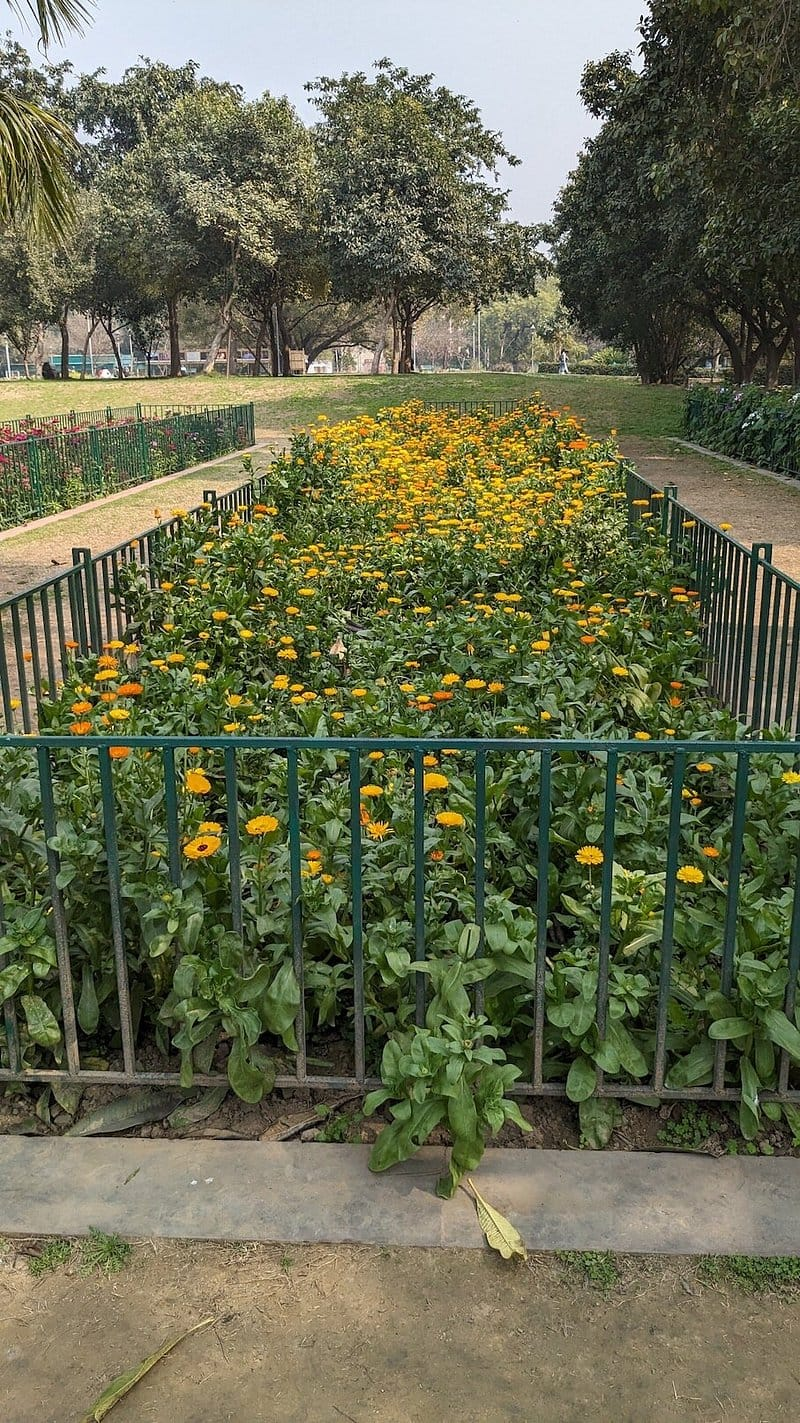
\includegraphics[width=\textwidth, height=5cm, keepaspectratio=false]{../Images/9.jpeg}
        \caption{Marigold beds}
    \end{subfigure}
    \hfill
    \begin{subfigure}[b]{0.32\textwidth}
        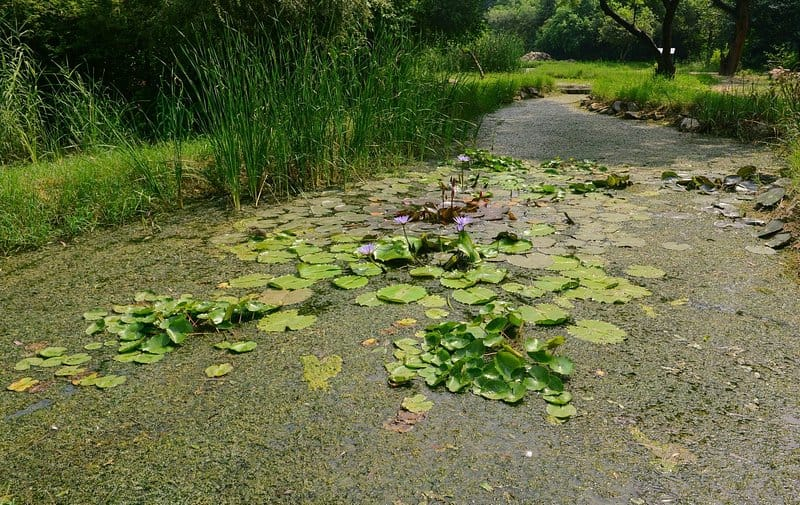
\includegraphics[width=\textwidth, height=5cm, keepaspectratio=false]{../Images/13.jpeg}
        \caption{Wetland with lotus}
    \end{subfigure}
    \caption{Flora and green cover at Sunder Nursery.}
    \label{fig:flora}
\end{figure}

\begin{figure}[H]
    \centering
    \begin{subfigure}[b]{0.32\textwidth}
        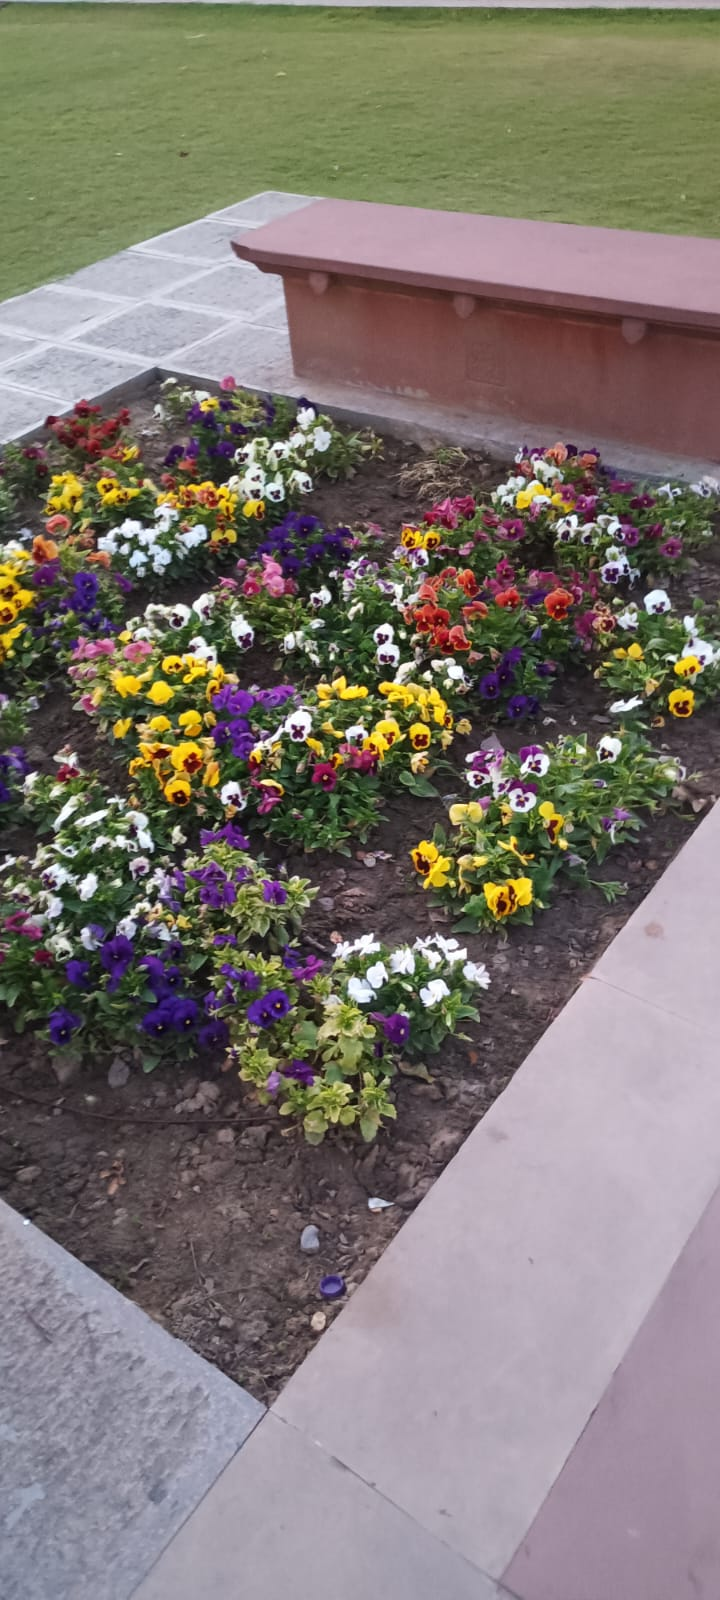
\includegraphics[width=\textwidth, height=5cm, keepaspectratio=false]{../Images/2.jpeg}
        \caption{Pansies}
    \end{subfigure}
    \hfill
    \begin{subfigure}[b]{0.32\textwidth}
        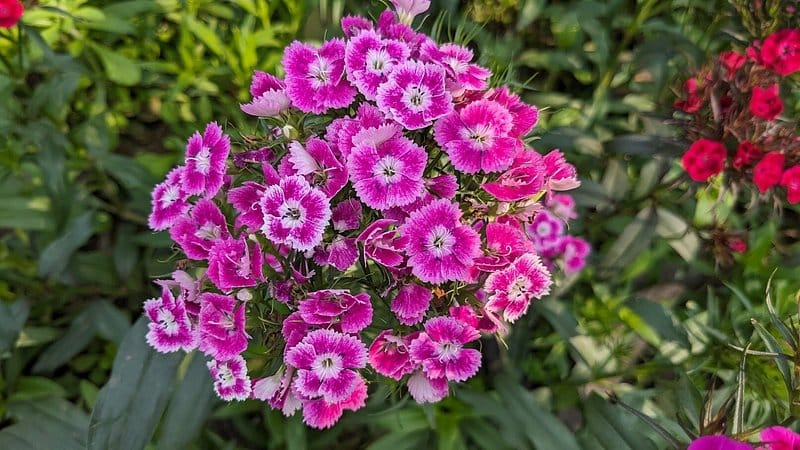
\includegraphics[width=\textwidth, height=5cm, keepaspectratio=false]{../Images/10.jpeg}
        \caption{Dianthus}
    \end{subfigure}
    \hfill
    \begin{subfigure}[b]{0.32\textwidth}
        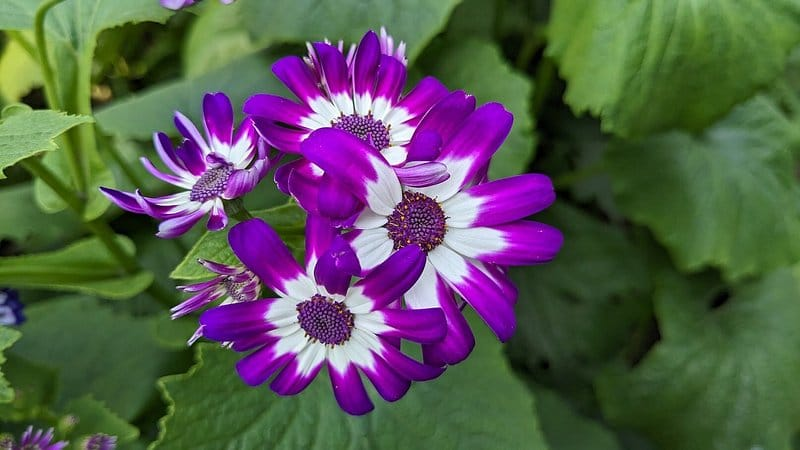
\includegraphics[width=\textwidth, height=5cm, keepaspectratio=false]{../Images/11.jpeg}
        \caption{Cineraria}
    \end{subfigure}
    \caption{Floral diversity at Sunder Nursery-a sample of the seasonal blooms observed during the visit.}
    \label{fig:flowers}
\end{figure}

% ════════════════════════════════════════════════════════════
%  3.  THEORETICAL FRAMEWORK
% ════════════════════════════════════════════════════════════
\section{Theoretical Framework}

\subsection{Total Economic Value}

Environmental economics distinguishes between several components of the value that people derive from a natural or heritage resource [2]. The \textbf{Total Economic Value (TEV)} framework captures all of these:

\begin{equation}
    \text{TEV} = \underbrace{\text{Use Value}}_{\text{direct enjoyment}} + \underbrace{\text{Non-Use Value}}_{\text{option + bequest + existence}}
    \label{eq:tev}
\end{equation}

\begin{itemize}[nosep]
    \item \textbf{Use Value:} The benefit a visitor gets from actually using the park-walking, picnicking, birdwatching, etc.
    \item \textbf{Option Value:} The amount people are willing to pay to keep the \textit{option} of visiting the park in the future, even if they are not sure they will.
    \item \textbf{Bequest Value:} The satisfaction people derive from knowing the park will be preserved for future generations.
    \item \textbf{Existence Value:} The value people place on simply knowing the park exists and is protected, regardless of whether they ever visit it.
\end{itemize}

Traditional market-based approaches (e.g., hedonic pricing, market pricing) can only capture use values that are reflected in market transactions. For resources like Sunder Nursery, where the entry fee (\rupee 20-30) vastly underestimates the true value, we need methods that can capture both use and non-use values.

\subsection{Contingent Valuation Method (CVM)}

The CVM is a \textbf{stated-preference technique} that creates a hypothetical market through a carefully designed survey [3]. Respondents are presented with a scenario describing the resource and are asked how much they would be willing to pay for its preservation or improvement.

As outlined in the course ebook [7], a good CVM survey has two major phases:
\begin{enumerate}[nosep]
    \item \textbf{Scenario Presentation:} The respondent is given enough information about the resource, its services, and the proposed action to make an informed judgment.
    \item \textbf{Valuation Question:} A carefully worded question reveals the respondent's willingness to pay (WTP). Closed-ended formats (with pre-specified bid amounts) are preferred over open-ended ones because they are more realistic and easier for respondents who may be unfamiliar with pricing environmental goods.
\end{enumerate}

The \textbf{payment vehicle}-the mechanism through which payment would be collected-is also important. It should feel realistic to respondents yet be neutral in its effect on their answers. In our study, we used an \textit{increased entry fee} as the payment vehicle, since visitors are already accustomed to paying an entry charge.

\subsection{Travel Cost Method (TCM)}

The TCM is a \textbf{revealed-preference technique} that infers the value of a recreational site from the actual travel expenditures visitors incur to reach it. The core idea is simple: the entry fee at most parks is nominal, but visitors reveal their true willingness to pay through the money and time they spend traveling.

As described in the case study of Lumpinee Park in Bangkok [1], the travel cost approach constructs an empirical demand function for the park. The \textbf{consumer surplus}-the area between the demand curve and the price line-measures the net benefit visitors receive over and above what they actually spend.

% ════════════════════════════════════════════════════════════
%  4.  METHODOLOGY
% ════════════════════════════════════════════════════════════
\section{Methodology}

\subsection{Survey Design}

We designed a bilingual (English-Hindi) questionnaire using Google Forms with 16 questions organized into six sections:

\begin{enumerate}[nosep]
    \item \textbf{Conservation \& Heritage (CVM Core):} What aspects of the park visitors value most (checkbox), and whether they would be willing to pay a higher entry fee for permanent conservation (Yes/No).
    \item \textbf{Contribution Details:} For those willing to pay-maximum extra amount (closed-ended: \rupee 10, \rupee 20, \rupee 50, or \rupee 100 per visit).
    \item \textbf{Protest Feedback:} For those not willing-their main reason.
    \item \textbf{Future Generations \& Ecology:} How important preservation is for future generations (bequest value), whether they would support conservation even if they could never visit again (existence value), and their rating of the park's current ecological condition.
    \item \textbf{Travel \& Accessibility (TCM Core):} Origin locality/PIN code, transport mode, whether sole destination, one-way travel cost, and travel time.
    \item \textbf{Demographics:} Visit frequency, age group, and occupation/income bracket.
\end{enumerate}

The form used \textbf{skip logic}: respondents who chose ``Yes'' for WTP were directed to the amount page, while those who chose ``No'' were directed to the protest-reason page. Both paths converged at the non-use value section.

\subsection{Data Collection}

\begin{itemize}[nosep]
    \item \textbf{Date:} Friday, 10 April 2026
    \item \textbf{Time:} 4:00 PM - 7:30 PM (evening visit)
    \item \textbf{Sample size:} 45 respondents
    \item \textbf{Method:} In-person, on-site survey using mobile phones
    \item \textbf{Location:} Various spots within Sunder Nursery
\end{itemize}

\begin{figure}[H]
    \centering
    \begin{subfigure}[b]{0.48\textwidth}
        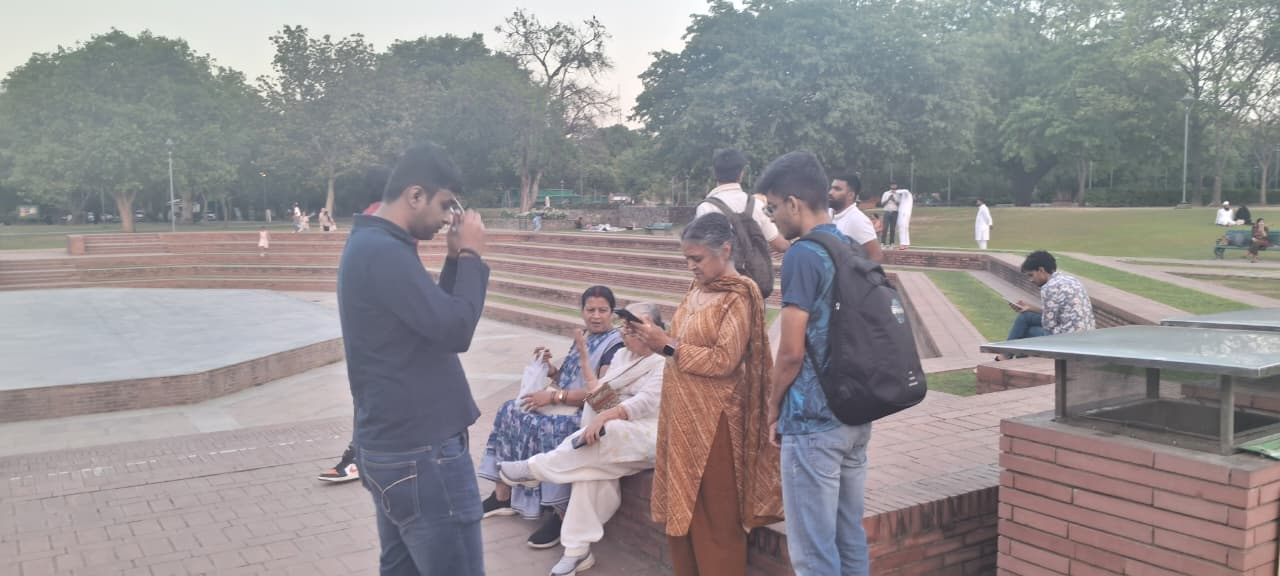
\includegraphics[width=\textwidth]{../Images/Review 6.jpeg}
        \caption{Conducting the survey with visitors}
    \end{subfigure}
    \hfill
    \begin{subfigure}[b]{0.48\textwidth}
        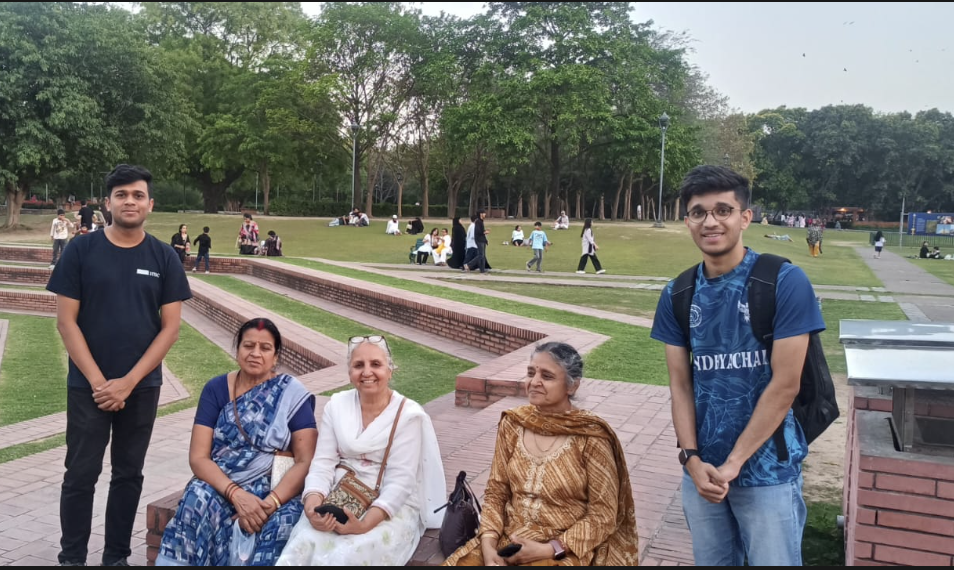
\includegraphics[width=\textwidth]{../Images/Review 5.jpeg}
        \caption{With respondents at the amphitheatre}
    \end{subfigure}
    \caption{Field survey in progress at Sunder Nursery.}
    \label{fig:field_survey}
\end{figure}

\begin{figure}[H]
    \centering
    \begin{subfigure}[b]{0.48\textwidth}
        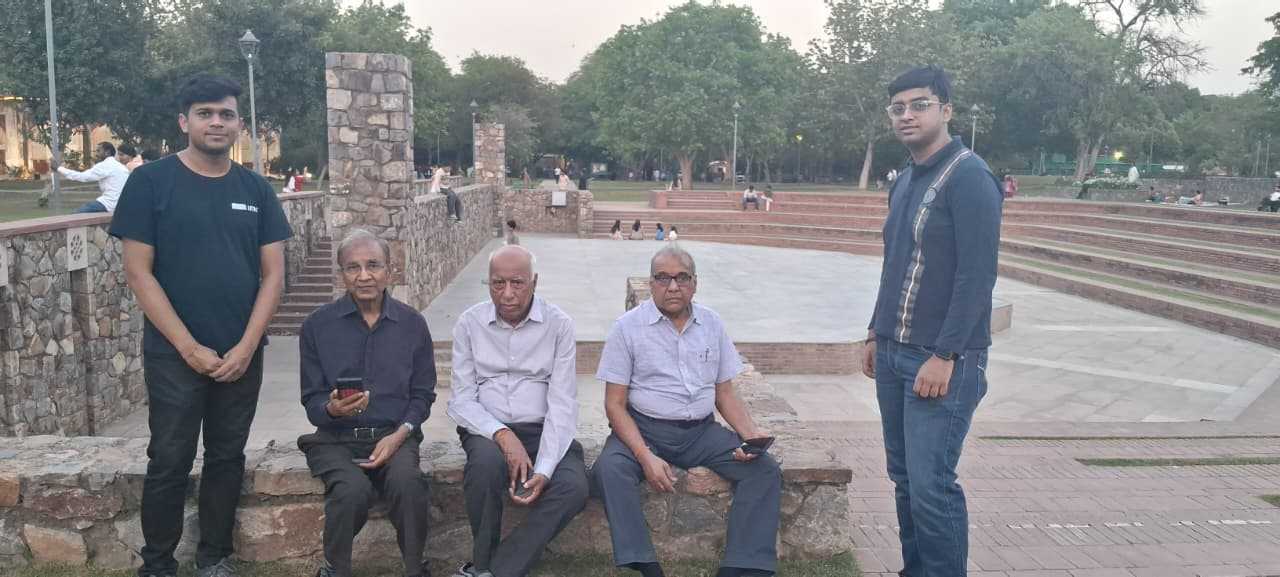
\includegraphics[width=\textwidth]{../Images/Review 3.jpeg}
        \caption{Interacting with elderly visitors}
    \end{subfigure}
    \hfill
    \begin{subfigure}[b]{0.48\textwidth}
        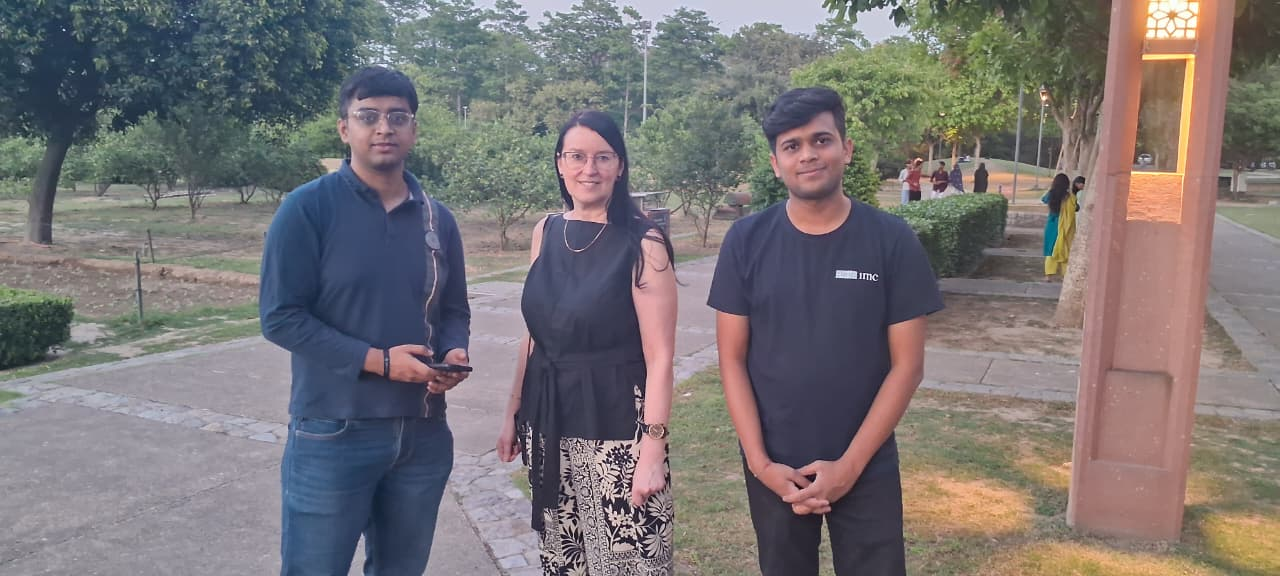
\includegraphics[width=\textwidth]{../Images/Review 7.jpeg}
        \caption{Surveying a visitor near the garden}
    \end{subfigure}
    \caption{Photographs from the field visit showing our team collecting survey responses.}
    \label{fig:field_photos}
\end{figure}

% ════════════════════════════════════════════════════════════
%  5.  RESULTS AND ANALYSIS
% ════════════════════════════════════════════════════════════
\section{Results and Analysis}

\subsection{Respondent Demographics}

Our sample of 45 respondents covered a broad cross-section of visitors. The largest group was young adults aged 18-35 (44.4\%), followed by the 36-60 age bracket (26.7\%). Students formed the biggest occupational category (35.6\%), reflecting the park's popularity among the college-going population in South Delhi.

\begin{figure}[H]
    \centering
    \begin{subfigure}[b]{0.48\textwidth}
        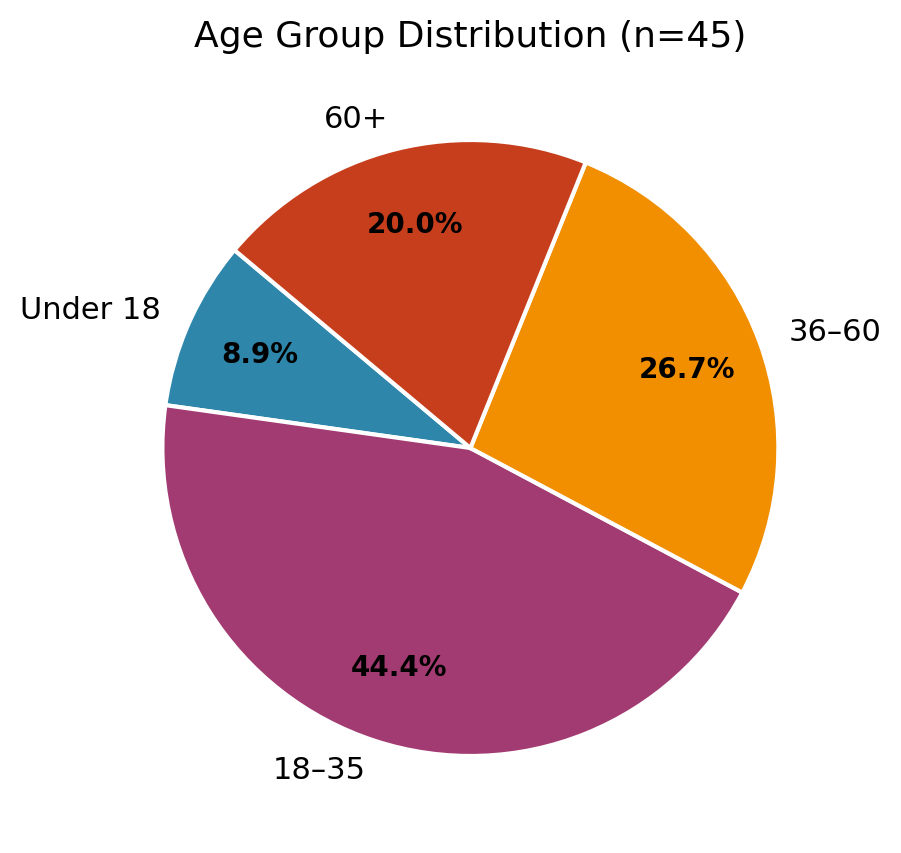
\includegraphics[width=\textwidth]{figures/01_age_distribution.png}
        \caption{Age group distribution}
    \end{subfigure}
    \hfill
    \begin{subfigure}[b]{0.48\textwidth}
        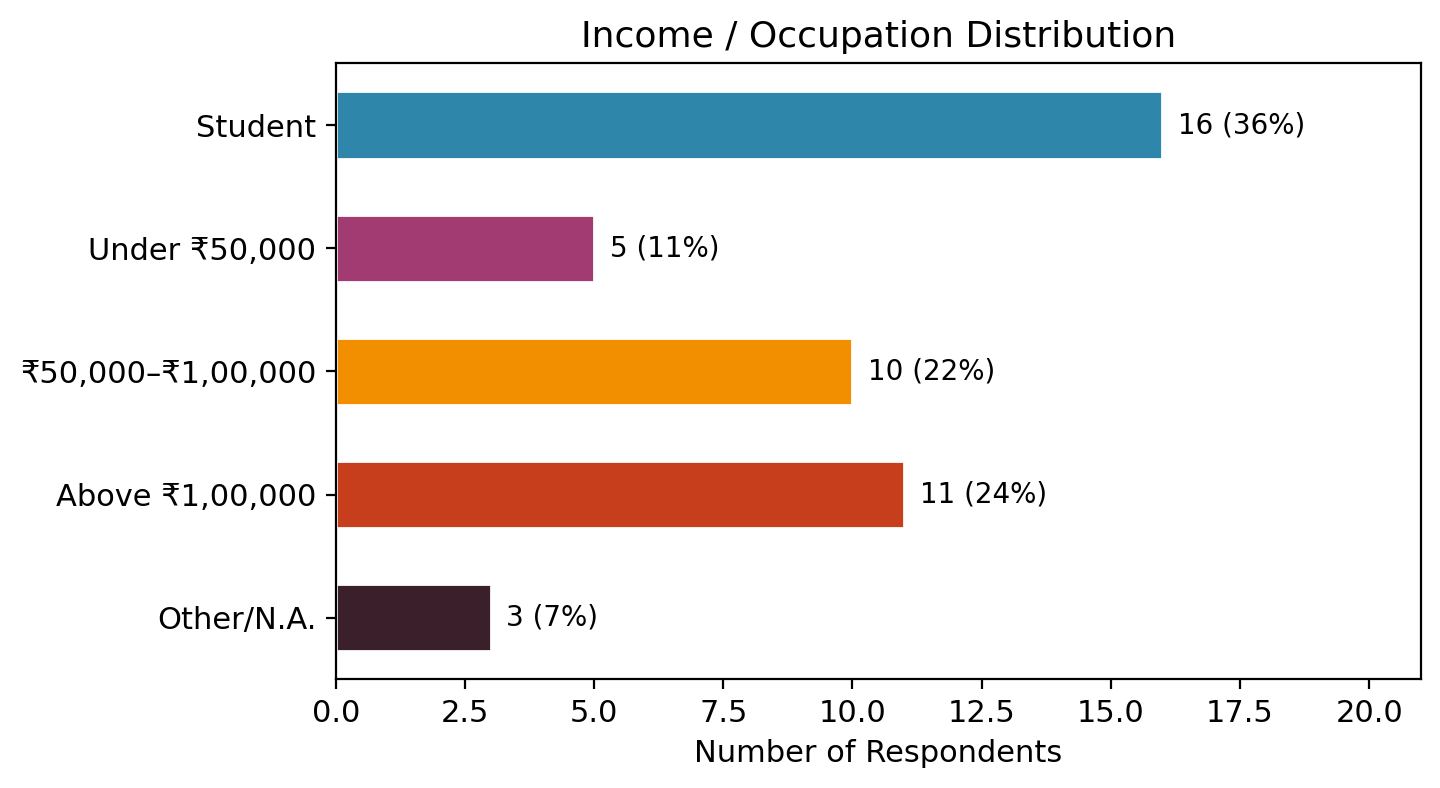
\includegraphics[width=\textwidth]{figures/02_income_distribution.png}
        \caption{Income/occupation distribution}
    \end{subfigure}
    \caption{Demographic profile of survey respondents (n=45).}
    \label{fig:demographics}
\end{figure}

In terms of visit frequency, 35.6\% were first-time visitors and 42.2\% visited rarely-indicating that the park attracts a large number of new or infrequent visitors alongside a smaller base of regulars.

\begin{figure}[H]
    \centering
    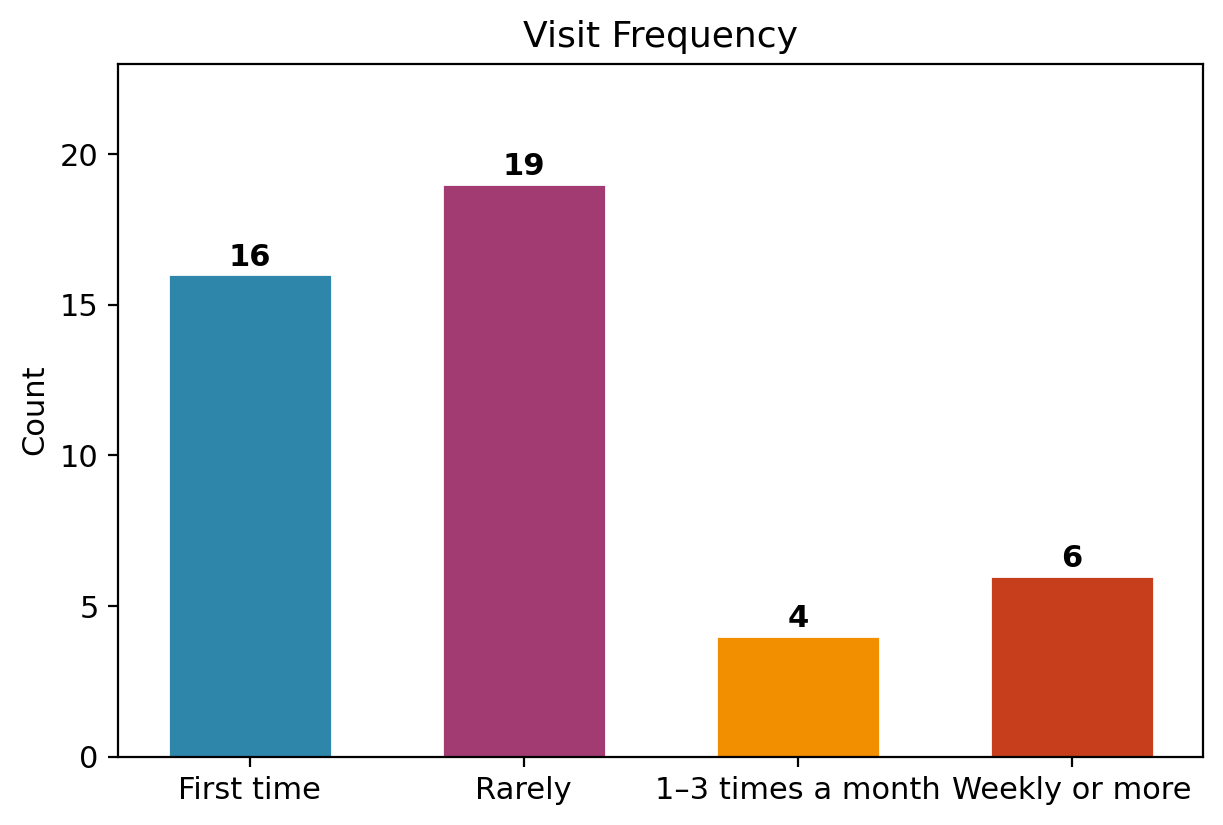
\includegraphics[width=0.65\textwidth]{figures/03_visit_frequency.png}
    \caption{Distribution of visit frequency among respondents.}
    \label{fig:visit_freq}
\end{figure}

\subsection{Aspects Most Valued}

Respondents were asked to select all aspects of Sunder Nursery that they value the most (multiple selections allowed). The results reveal that \textbf{aesthetic and scenic beauty} dominates with 84.4\%, followed by heritage monuments (55.6\%) and protection of native plants and birds (46.7\%).

\begin{figure}[H]
    \centering
    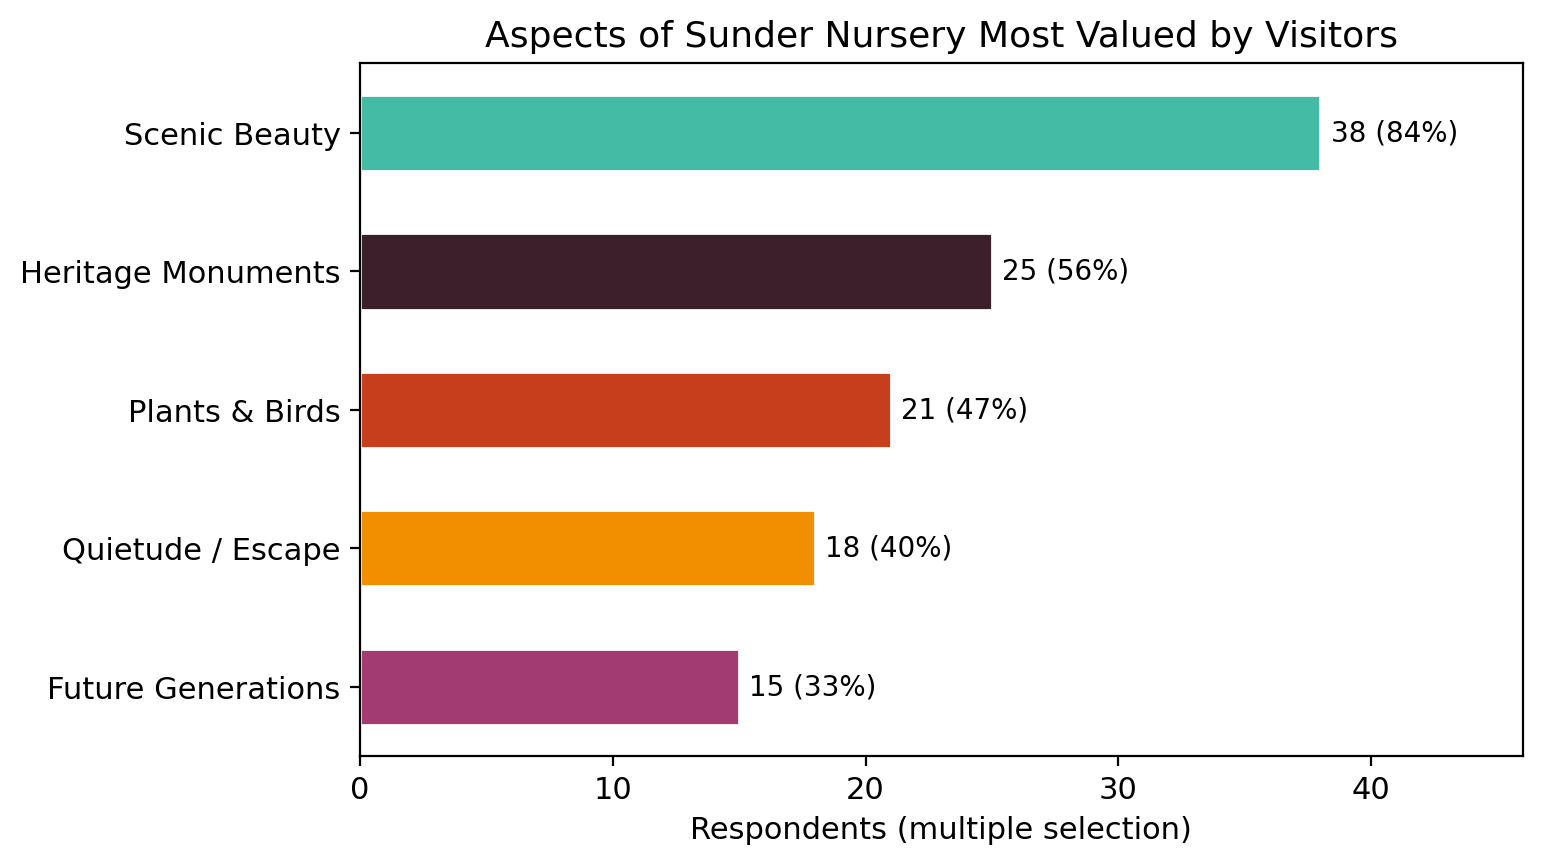
\includegraphics[width=0.75\textwidth]{figures/04_aspects_valued.png}
    \caption{Aspects of Sunder Nursery most valued by visitors.}
    \label{fig:aspects}
\end{figure}

The fact that ``Availability for future generations'' was selected by a third of all respondents-even though it was the last option in the list-is a strong signal of latent bequest value among the visitor population.

\subsection{CVM Analysis: Willingness to Pay}

\subsubsection{Overall WTP}

When asked whether they would be willing to pay a slightly higher entry fee to guarantee permanent protection of the park's monuments, gardens, and birds, \textbf{66.7\% of respondents said Yes} and 33.3\% said No.

\begin{figure}[H]
    \centering
    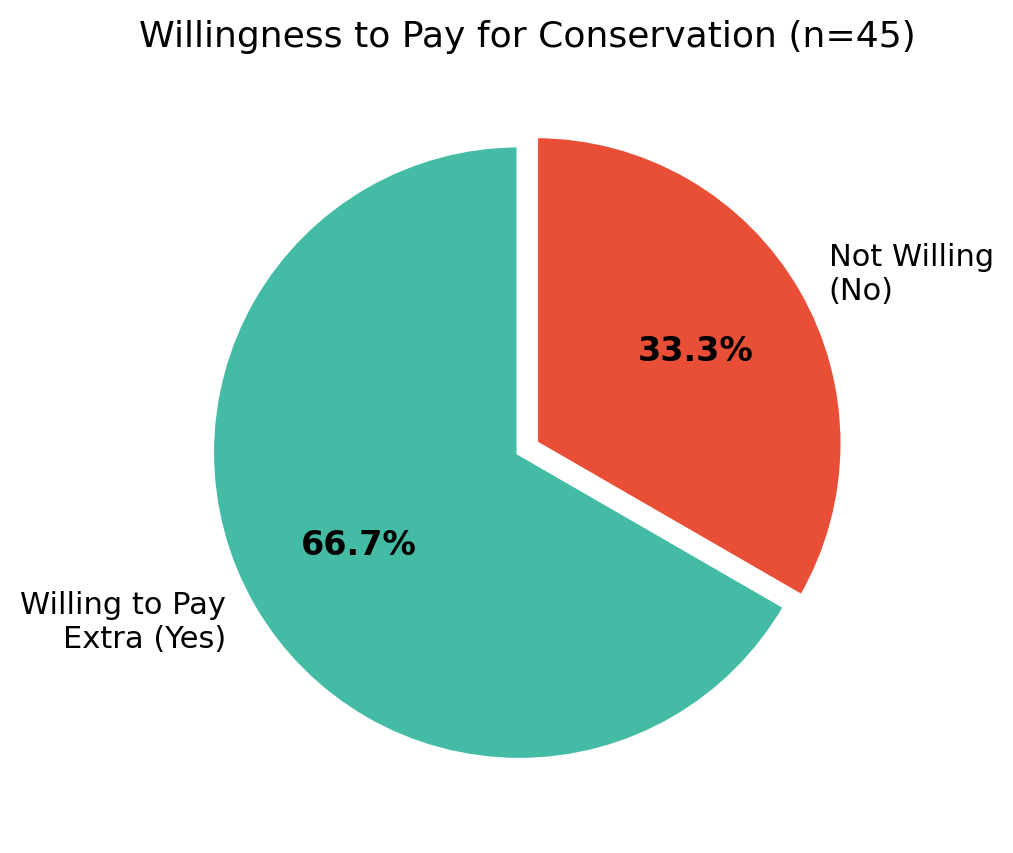
\includegraphics[width=0.55\textwidth]{figures/05_wtp_pie.png}
    \caption{Willingness to pay a higher entry fee for conservation.}
    \label{fig:wtp_pie}
\end{figure}

\subsubsection{WTP Amount Distribution}

Among the 30 respondents willing to pay extra, the most frequently chosen amount was \rupee 20 (43\%), followed by \rupee 50 (27\%), \rupee 100 (17\%), and \rupee 10 (13\%).

\begin{figure}[H]
    \centering
    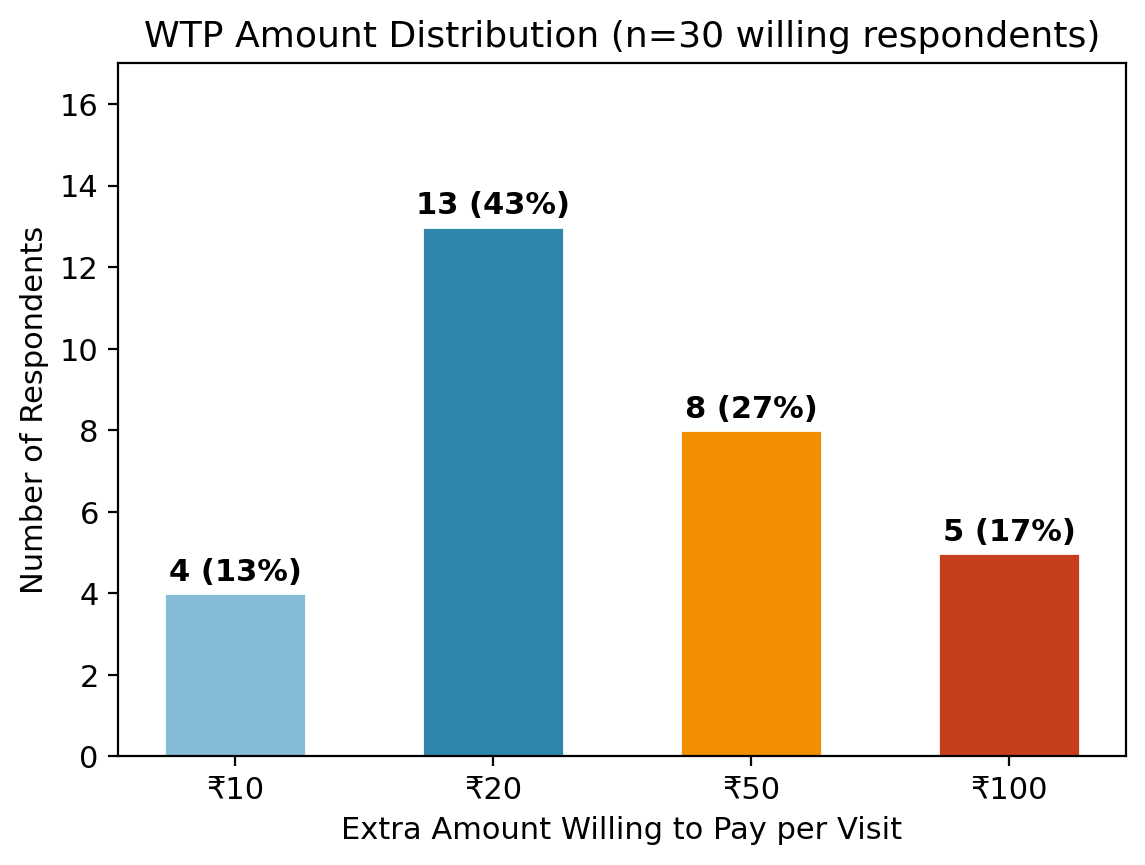
\includegraphics[width=0.65\textwidth]{figures/06_wtp_amount_distribution.png}
    \caption{Distribution of maximum extra amount willing to pay per visit.}
    \label{fig:wtp_amount}
\end{figure}

The key CVM statistics are:

\begin{table}[H]
\centering
\caption{Summary of CVM willingness-to-pay estimates.}
\label{tab:wtp_summary}
\begin{tabular}{lr}
\toprule
\textbf{Statistic} & \textbf{Value} \\
\midrule
Respondents willing to pay extra            & 30 / 45 (66.7\%) \\
Mean WTP (among willing respondents)        & \rupee 40.0 per visit \\
Median WTP (among willing respondents)      & \rupee 20 per visit \\
Overall Mean WTP (including zeros for ``No'') & \rupee 26.7 per visit \\
Estimated annual visitors                   & $\sim$15,00,000 \\
\textbf{Aggregate annual WTP}               & \textbf{\rupee 4.00 crore} \\
\bottomrule
\end{tabular}
\end{table}

\subsubsection{WTP Cumulative Distribution}

Figure~\ref{fig:wtp_cdf} shows the survival function (reverse CDF) of willingness to pay. At \rupee 0, 100\% of respondents are willing to pay at least that much. The function drops to about 67\% at any positive amount (the WTP=Yes fraction), then gradually declines-roughly 31\% would pay \rupee 50 or more, and 13\% would pay \rupee 100.

\begin{figure}[H]
    \centering
    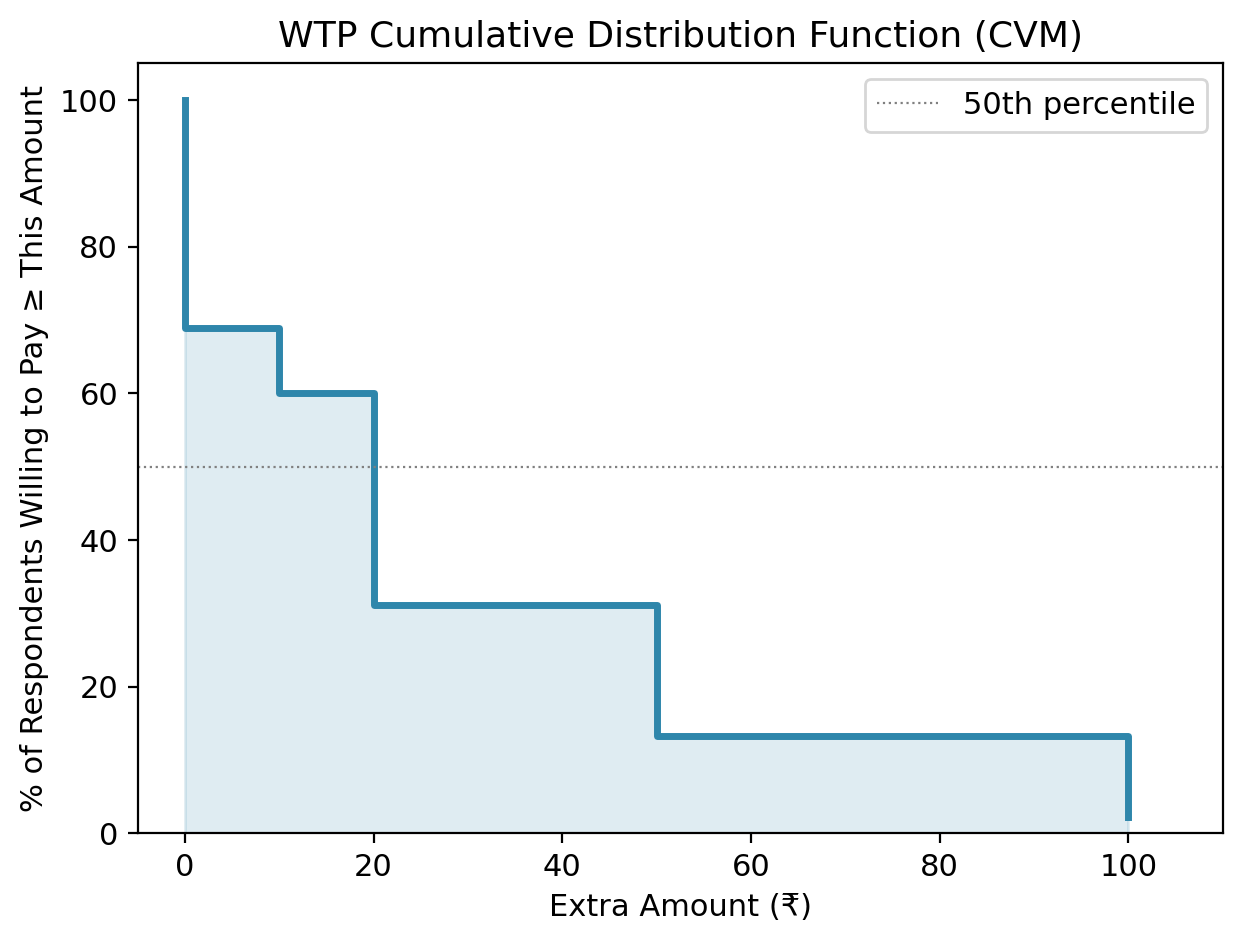
\includegraphics[width=0.65\textwidth]{figures/23_wtp_cdf.png}
    \caption{WTP cumulative distribution function-the area under this curve represents the aggregate WTP.}
    \label{fig:wtp_cdf}
\end{figure}

\subsubsection{Protest Bid Analysis}

Among the 15 respondents who chose \textit{not} to pay extra, the reasons were:
\begin{itemize}[nosep]
    \item 40\% said they did not think the park is worth paying more for
    \item 33\% said the government/management should bear the cost, not visitors
    \item 27\% said they simply cannot afford to pay more
\end{itemize}

\begin{figure}[H]
    \centering
    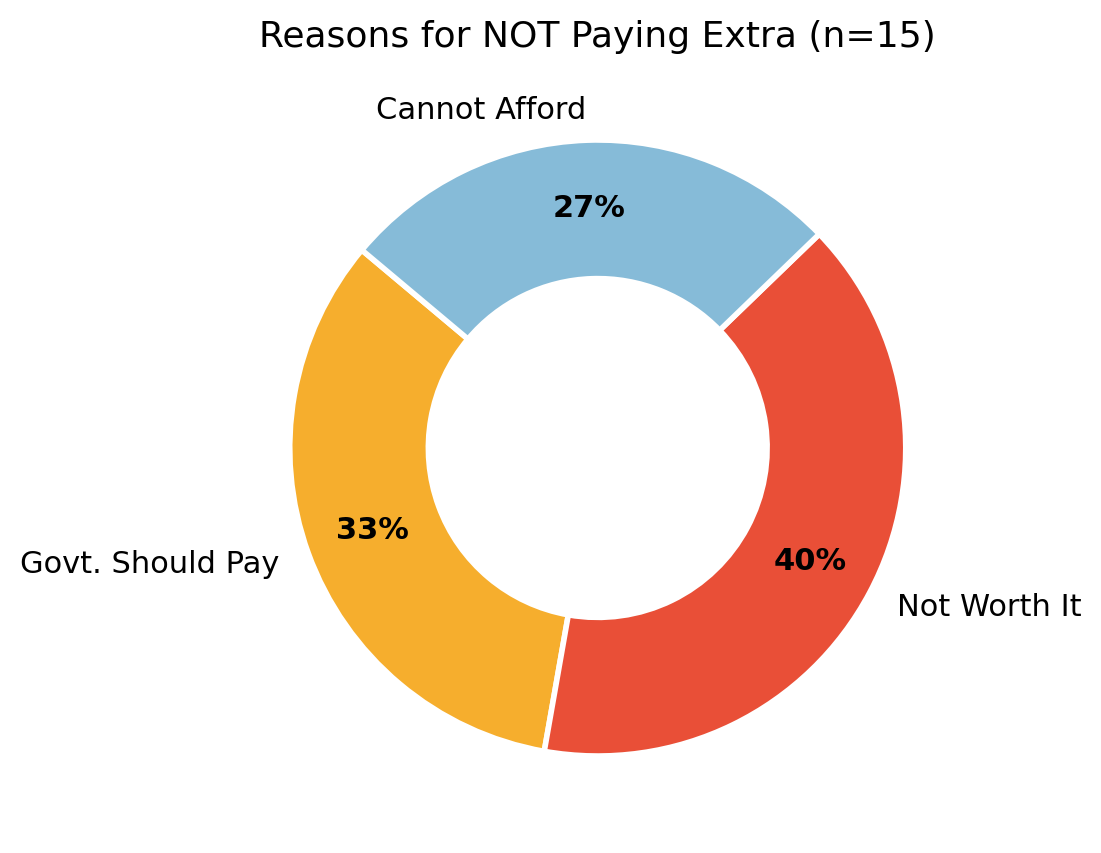
\includegraphics[width=0.55\textwidth]{figures/07_protest_bids.png}
    \caption{Reasons given by respondents who chose not to pay extra.}
    \label{fig:protest}
\end{figure}

The ``government should pay'' response is what the CVM literature calls a \textbf{protest bid}-these respondents are not saying the park has no value; they are objecting to the payment vehicle (user fees). If we treat these 5 protest bids as non-informative and exclude them, the adjusted WTP rate rises to $\frac{30}{40} = 75\%$.

\subsection{Non-Use Value Analysis}

\subsubsection{Bequest Value}

When asked how important it is to preserve Sunder Nursery for future generations, an overwhelming \textbf{68.9\%} said ``Very important'' and 26.7\% said ``Somewhat important.'' Only 4.4\% said it was not important.

\begin{figure}[H]
    \centering
    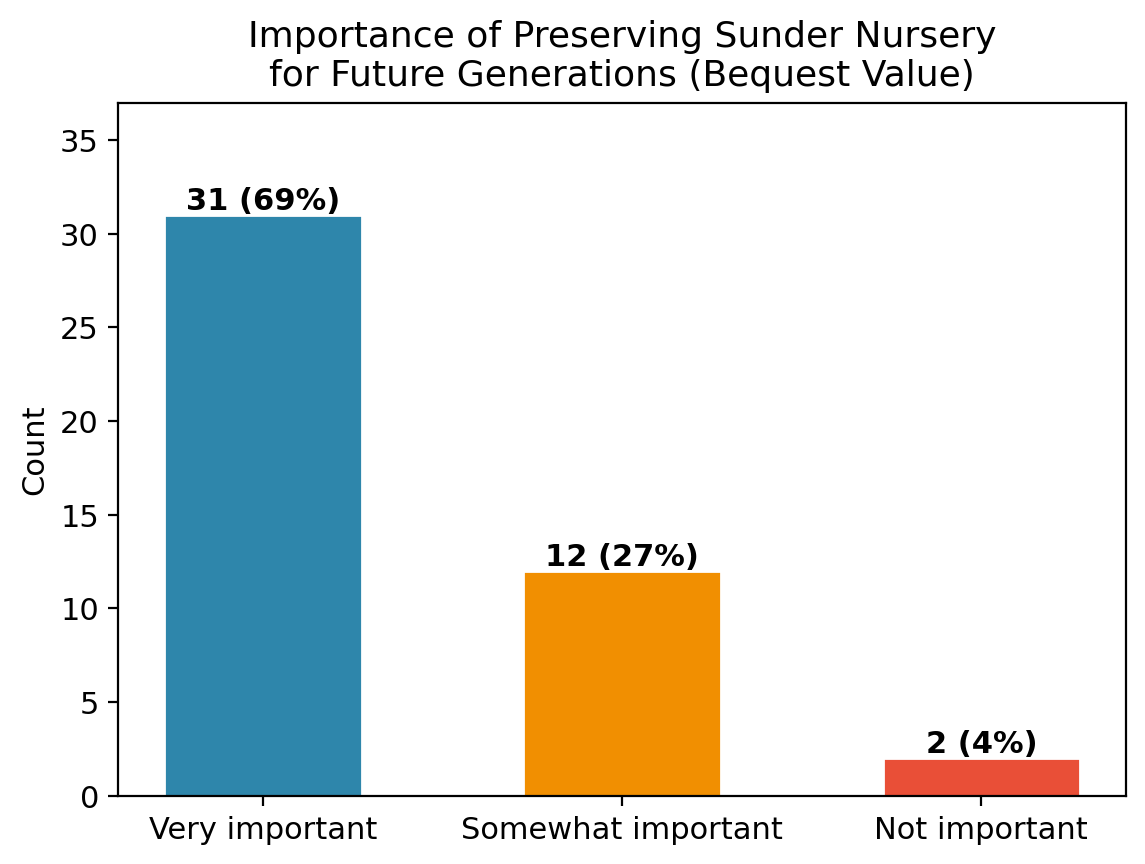
\includegraphics[width=0.6\textwidth]{figures/08_future_importance.png}
    \caption{Importance of preserving Sunder Nursery for future generations (bequest value).}
    \label{fig:bequest}
\end{figure}

\subsubsection{Existence Value}

An even stronger signal came from the existence-value question: \textbf{82.2\%} of respondents said they would support conservation of the park even if they could \textit{never visit it again}.

\begin{figure}[H]
    \centering
    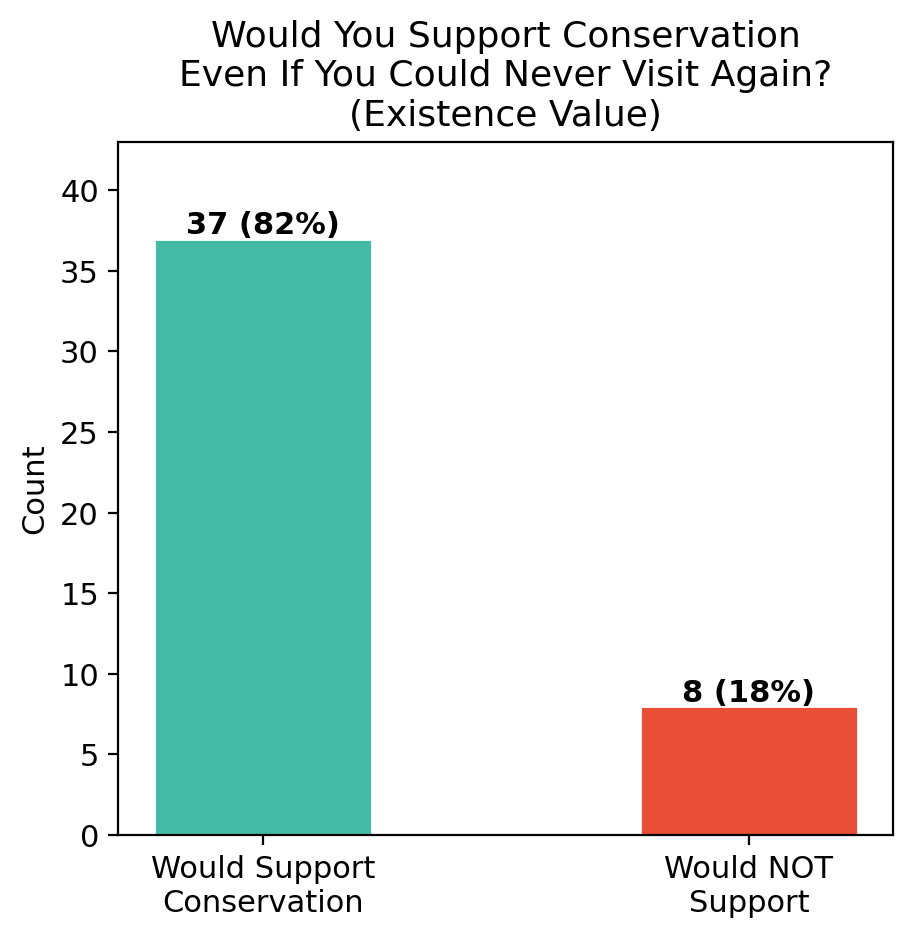
\includegraphics[width=0.55\textwidth]{figures/09_existence_value.png}
    \caption{Support for conservation even without the possibility of future visits (existence value).}
    \label{fig:existence}
\end{figure}

These results are consistent with the Kalamazoo Nature Center case study discussed in the course ebook [7], where non-use values were found to be a significant component of total value.

\begin{figure}[H]
    \centering
    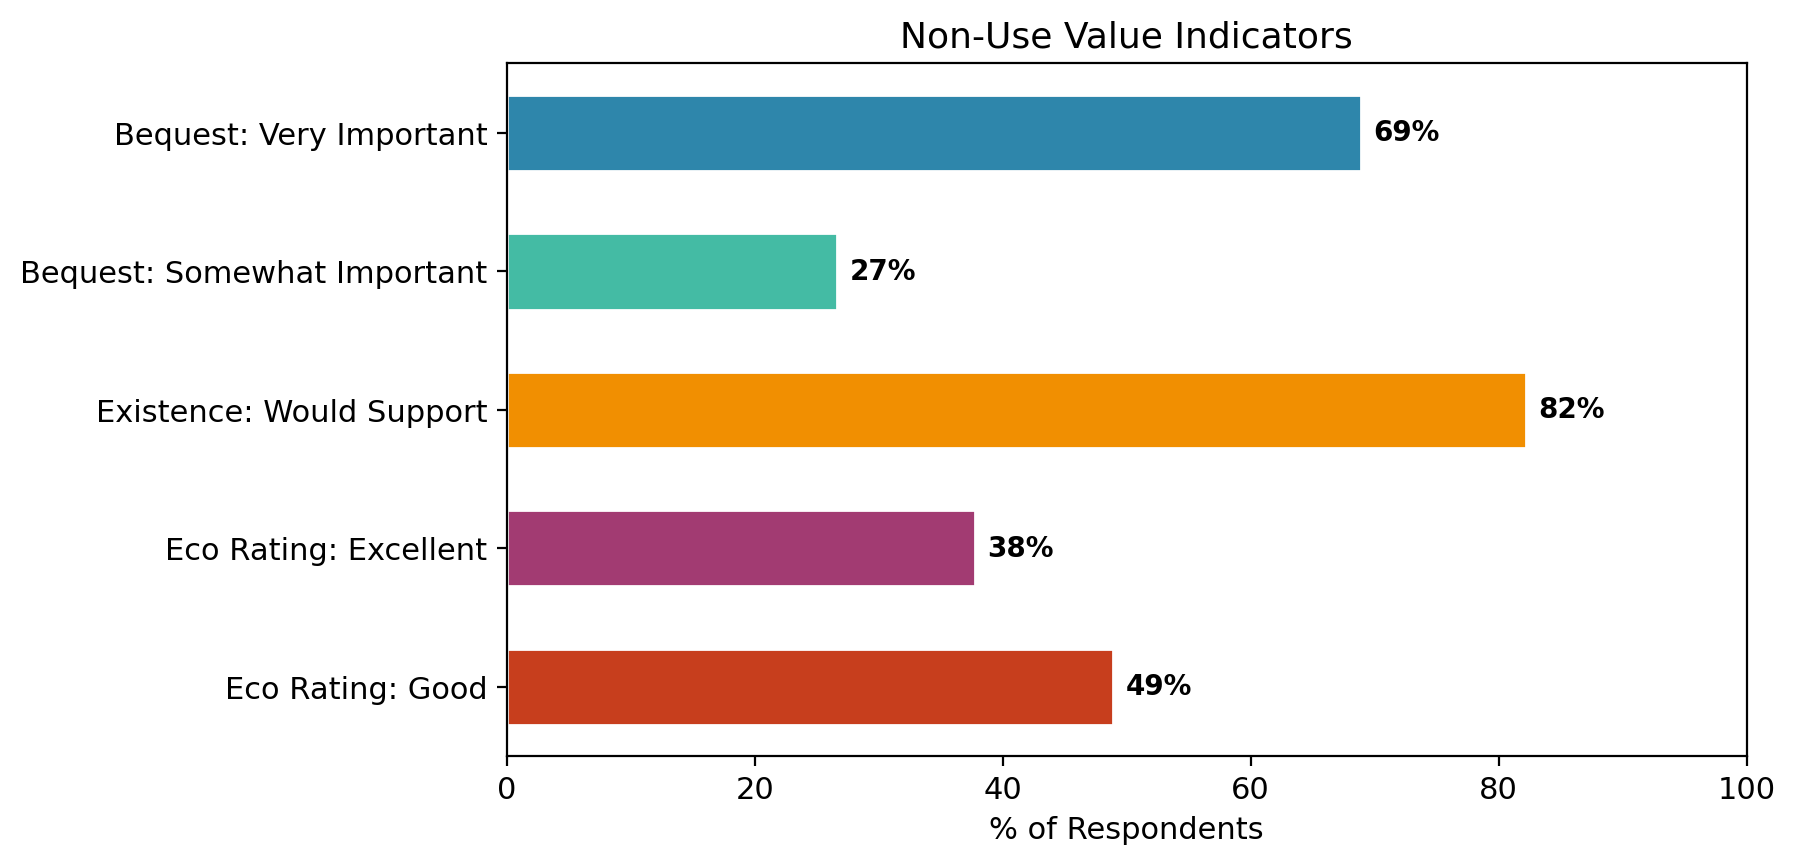
\includegraphics[width=0.75\textwidth]{figures/20_nonuse_value_summary.png}
    \caption{Summary of non-use value indicators.}
    \label{fig:nonuse_summary}
\end{figure}

\subsection{Ecological Condition Rating}

Visitors were asked to rate the current ecological condition of Sunder Nursery. The results strongly validate the success of the Aga Khan Trust restoration: \textbf{37.8\% rated it ``Excellent''} and \textbf{48.9\% rated it ``Good.''} Only 13.3\% rated it ``Average,'' and no respondent rated it ``Poor.''

\begin{figure}[H]
    \centering
    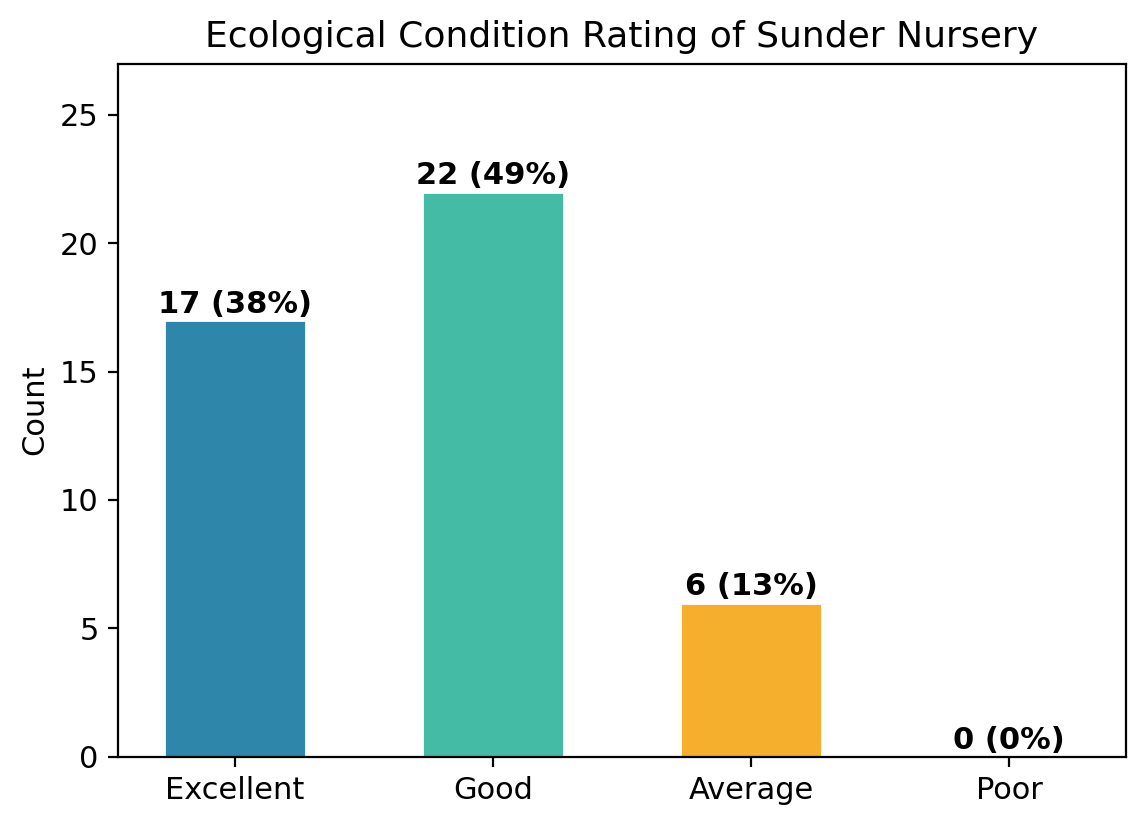
\includegraphics[width=0.6\textwidth]{figures/10_ecological_condition.png}
    \caption{Ecological condition rating by visitors.}
    \label{fig:eco_rating}
\end{figure}

\subsection{TCM Analysis: Travel Cost and Consumer Surplus}

\subsubsection{Transport Mode and Travel Cost}

The most common mode of transport was auto/taxi/cab (40\%), followed by personal car or bike (31.1\%) and metro/bus (20\%). Only 8.9\% walked, indicating that the park draws visitors from across the city rather than just the immediate neighborhood.

\begin{figure}[H]
    \centering
    \begin{subfigure}[b]{0.48\textwidth}
        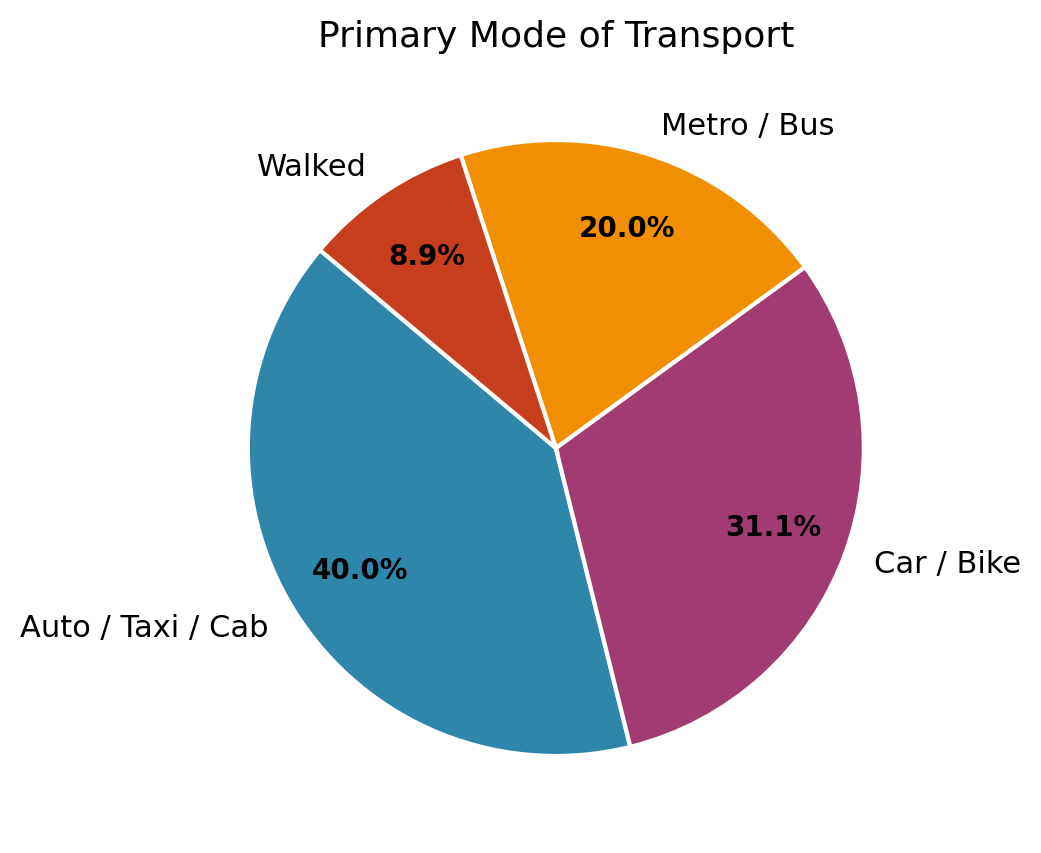
\includegraphics[width=\textwidth]{figures/11_transport_mode.png}
        \caption{Transport mode}
    \end{subfigure}
    \hfill
    \begin{subfigure}[b]{0.48\textwidth}
        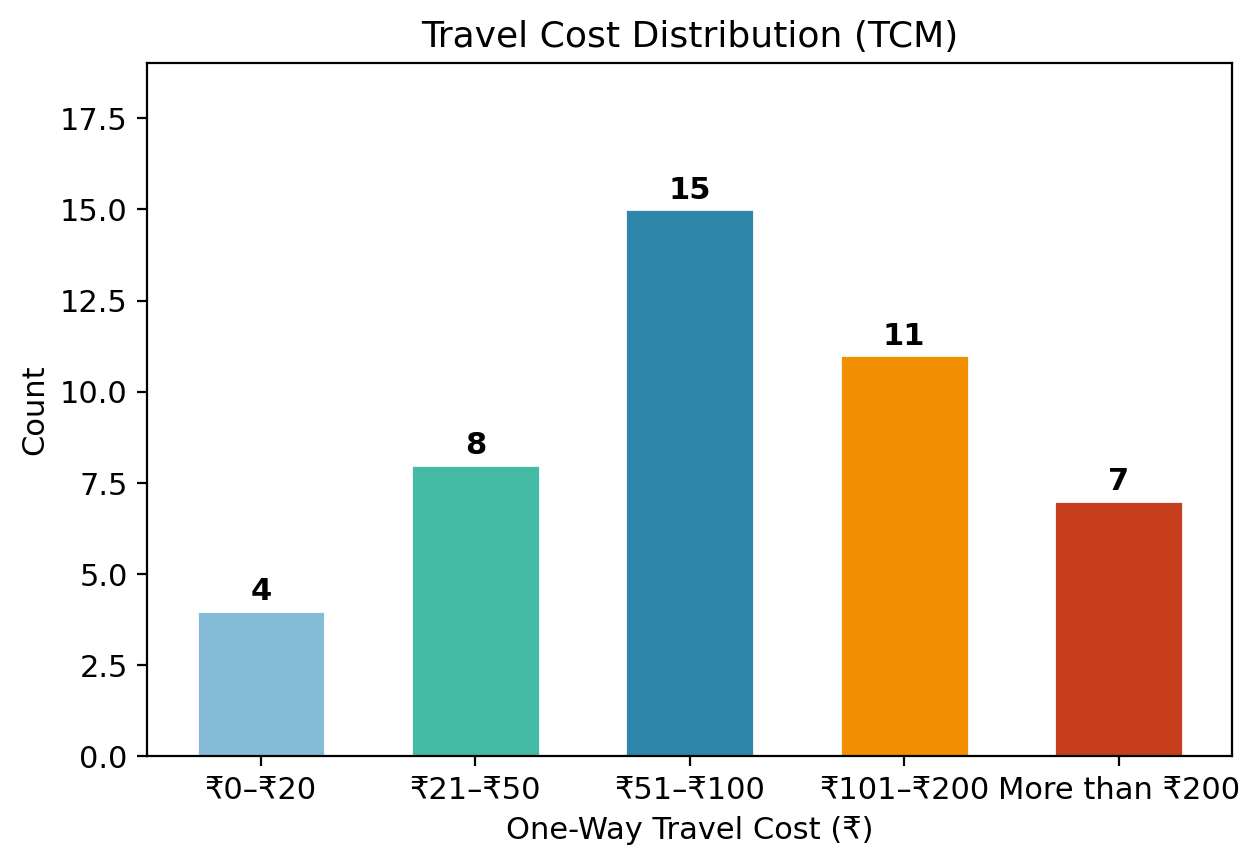
\includegraphics[width=\textwidth]{figures/12_travel_cost.png}
        \caption{One-way travel cost}
    \end{subfigure}
    \caption{Travel characteristics of visitors (TCM data).}
    \label{fig:tcm_data}
\end{figure}

The mean one-way travel cost was \rupee 107.7, giving a round-trip cost of \rupee 215.3. The largest share of visitors (33.3\%) spent \rupee 51-100, while 15.6\% spent more than \rupee 200 one-way.

\subsubsection{Travel Time and Trip Purpose}

Over half the visitors (51.1\%) took 31-60 minutes to reach the park. Interestingly, 53.3\% said they were also visiting nearby places (notably Humayun's Tomb), which means the travel cost for these visitors is shared across multiple destinations.

\begin{figure}[H]
    \centering
    \begin{subfigure}[b]{0.48\textwidth}
        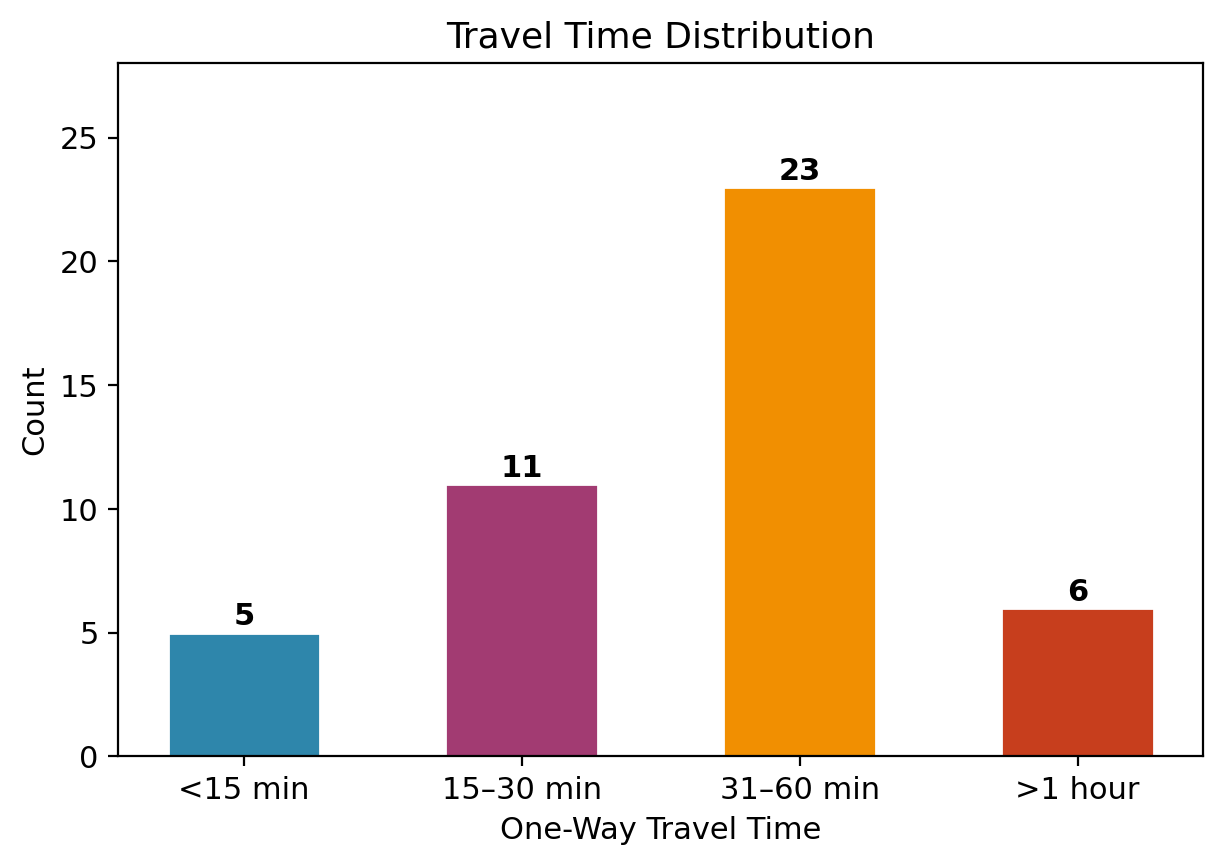
\includegraphics[width=\textwidth]{figures/13_travel_time.png}
        \caption{Travel time (one-way)}
    \end{subfigure}
    \hfill
    \begin{subfigure}[b]{0.48\textwidth}
        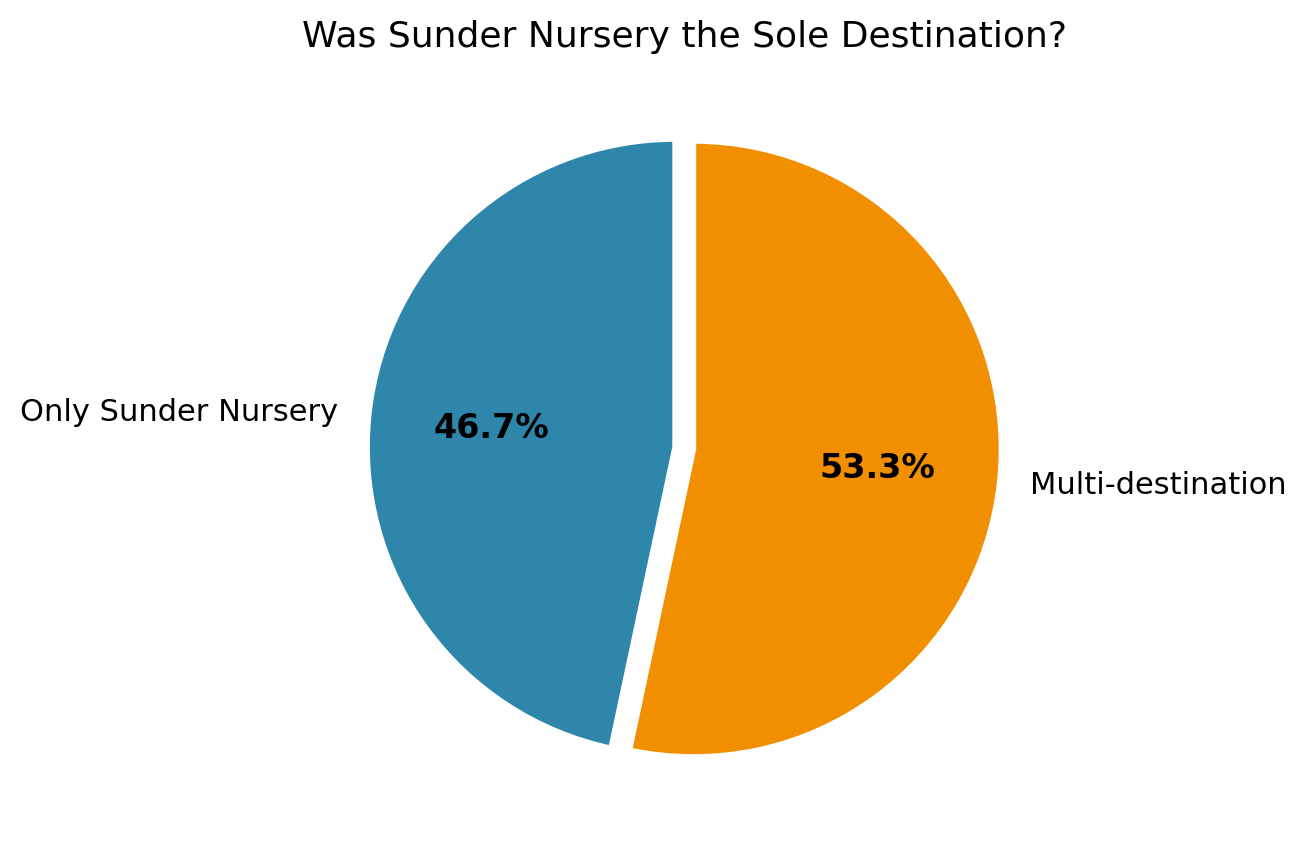
\includegraphics[width=\textwidth]{figures/14_sole_destination.png}
        \caption{Sole vs.\ multi-destination trip}
    \end{subfigure}
    \caption{Travel time and trip purpose.}
    \label{fig:travel_details}
\end{figure}

\subsubsection{Demand Curve and Consumer Surplus}

Using the zonal travel cost approach, we constructed a demand curve for Sunder Nursery (Figure~\ref{fig:consumer_surplus}). The downward-sloping curve confirms the theoretical expectation: as travel cost increases, the proportion of visitors willing to travel that distance decreases. The shaded area between the demand curve and the current entry fee (\rupee 30) represents the \textbf{consumer surplus}-the benefit visitors enjoy over and above what they actually pay.

\begin{figure}[H]
    \centering
    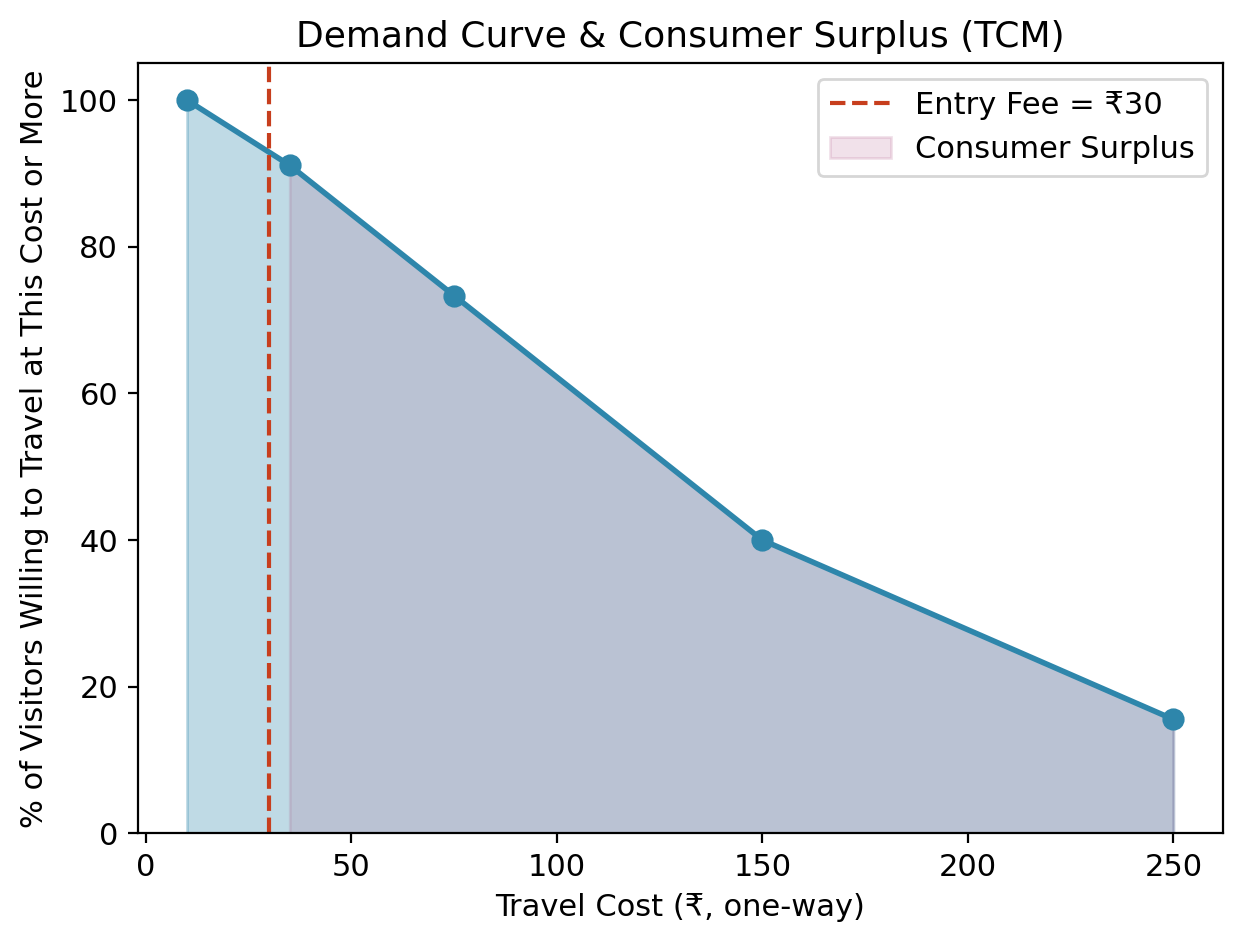
\includegraphics[width=0.7\textwidth]{figures/19_consumer_surplus.png}
    \caption{Demand curve and consumer surplus estimated via the Travel Cost Method.}
    \label{fig:consumer_surplus}
\end{figure}

\begin{table}[H]
\centering
\caption{Travel Cost Method estimates.}
\label{tab:tcm}
\begin{tabular}{lr}
\toprule
\textbf{Statistic} & \textbf{Value} \\
\midrule
Mean one-way travel cost              & \rupee 107.7 \\
Mean round-trip travel cost           & \rupee 215.3 \\
Consumer surplus per visitor          & \rupee 142.3 \\
Estimated annual visitors             & $\sim$15,00,000 \\
\textbf{Annual consumer surplus}      & \textbf{\rupee 21.35 crore} \\
\bottomrule
\end{tabular}
\end{table}

\subsection{Cross-Tabulations}

\subsubsection{Income vs.\ WTP}

An interesting pattern emerges when we cross-tabulate income with WTP. Students showed the highest WTP rate (81\%), which may seem counter-intuitive given their lower income. However, this is consistent with CVM literature, which notes that environmental concern and emotional attachment to a resource can outweigh income effects, especially when the payment vehicle (a small entry-fee increase) is modest.

\begin{figure}[H]
    \centering
    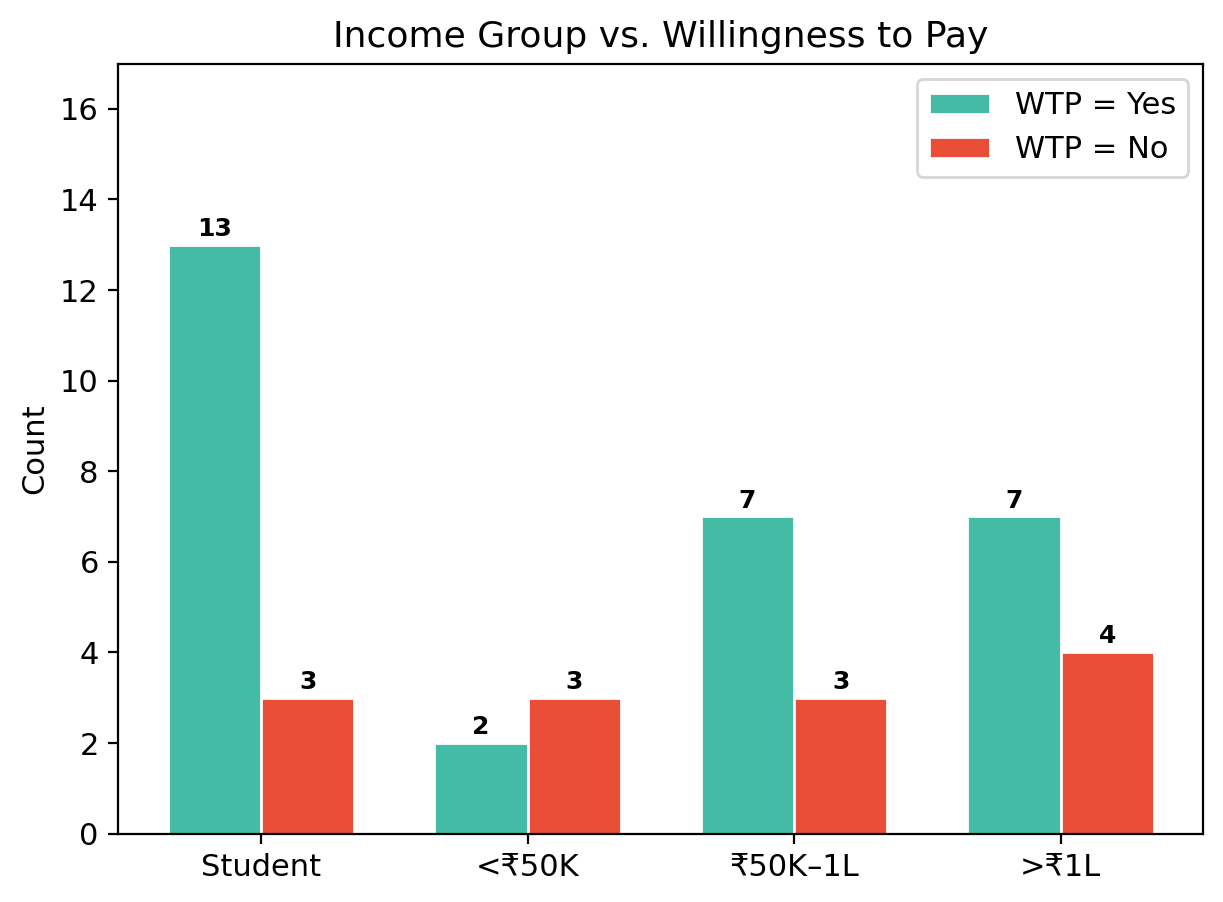
\includegraphics[width=0.65\textwidth]{figures/15_income_vs_wtp.png}
    \caption{Income group vs.\ willingness to pay.}
    \label{fig:income_wtp}
\end{figure}

\subsubsection{Age vs.\ WTP}

All four respondents under 18 were willing to pay extra (100\%), while the WTP rate decreases with age, dropping to 44\% for the 60+ group. Older visitors, while deeply appreciative of the park, may be more sensitive to price increases on principle.

\begin{figure}[H]
    \centering
    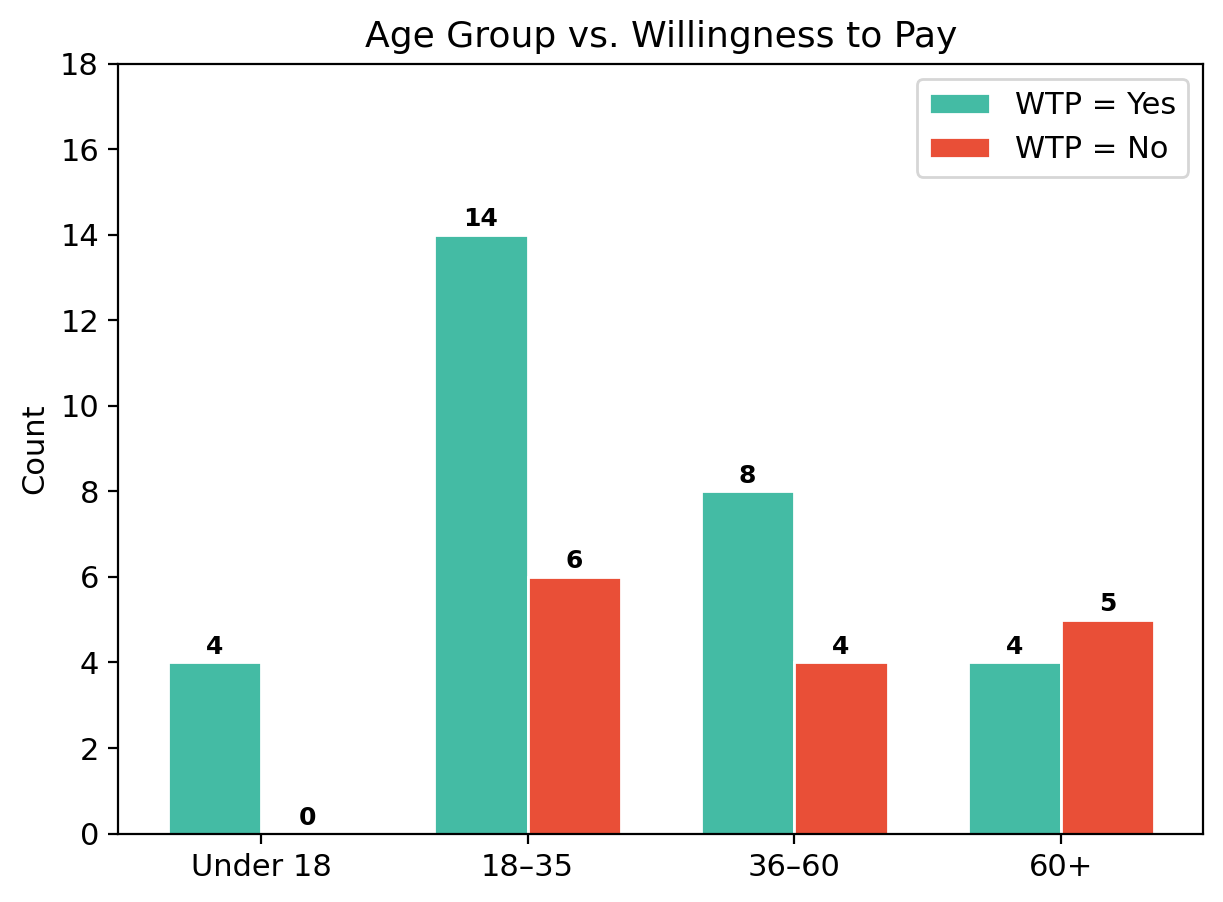
\includegraphics[width=0.65\textwidth]{figures/16_age_vs_wtp.png}
    \caption{Age group vs.\ willingness to pay.}
    \label{fig:age_wtp}
\end{figure}

\subsubsection{WTP Amount by Income Group}

Among those willing to pay, Figure~\ref{fig:amt_income} shows how the chosen amounts vary across income groups. Higher-income groups tend to choose larger amounts (\rupee 50-100), while students cluster around \rupee 10-20.

\begin{figure}[H]
    \centering
    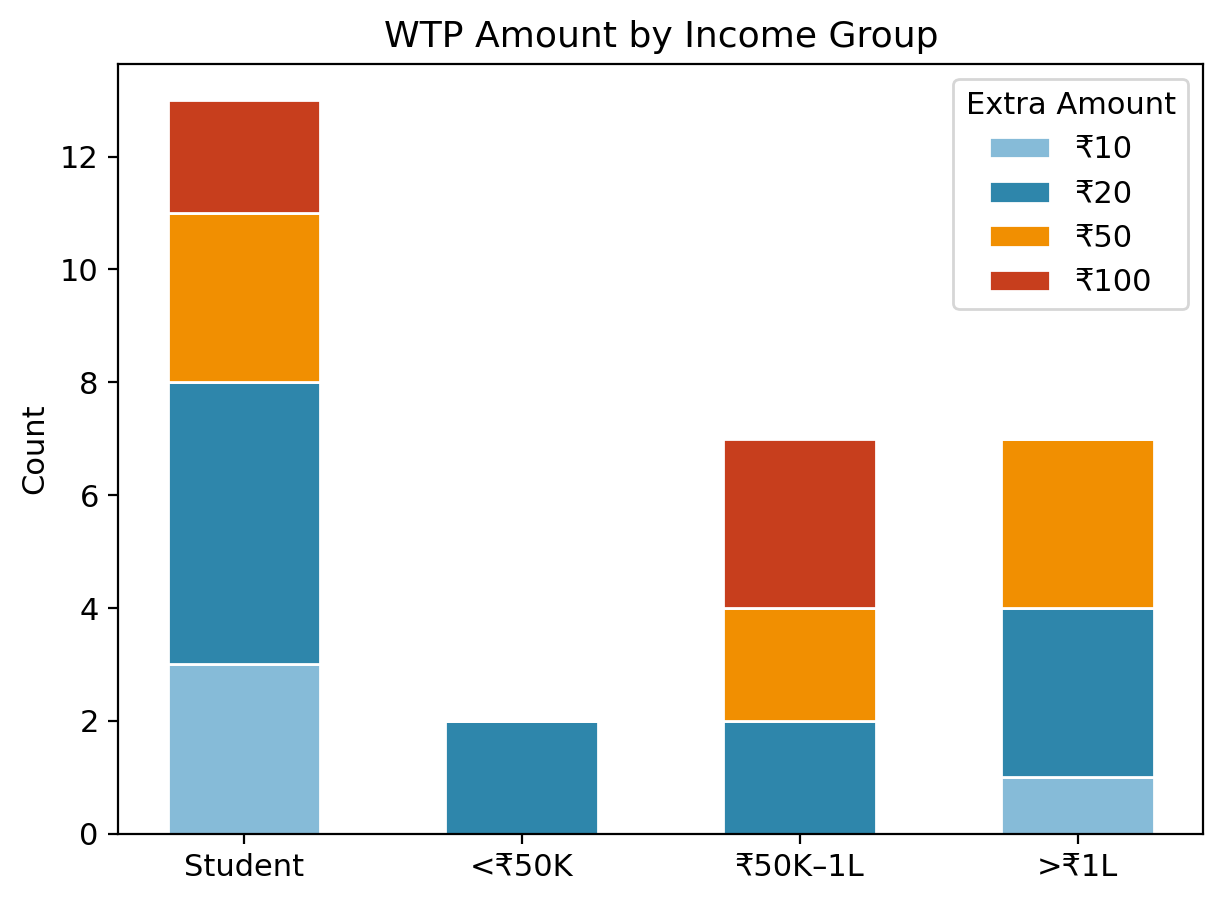
\includegraphics[width=0.65\textwidth]{figures/17_amount_vs_income.png}
    \caption{WTP amount distribution by income group.}
    \label{fig:amt_income}
\end{figure}

\subsubsection{Ecological Rating vs.\ WTP}

Respondents who rated the park's ecological condition as ``Excellent'' were more likely to pay extra, suggesting that a positive visitor experience reinforces conservation support.

\begin{figure}[H]
    \centering
    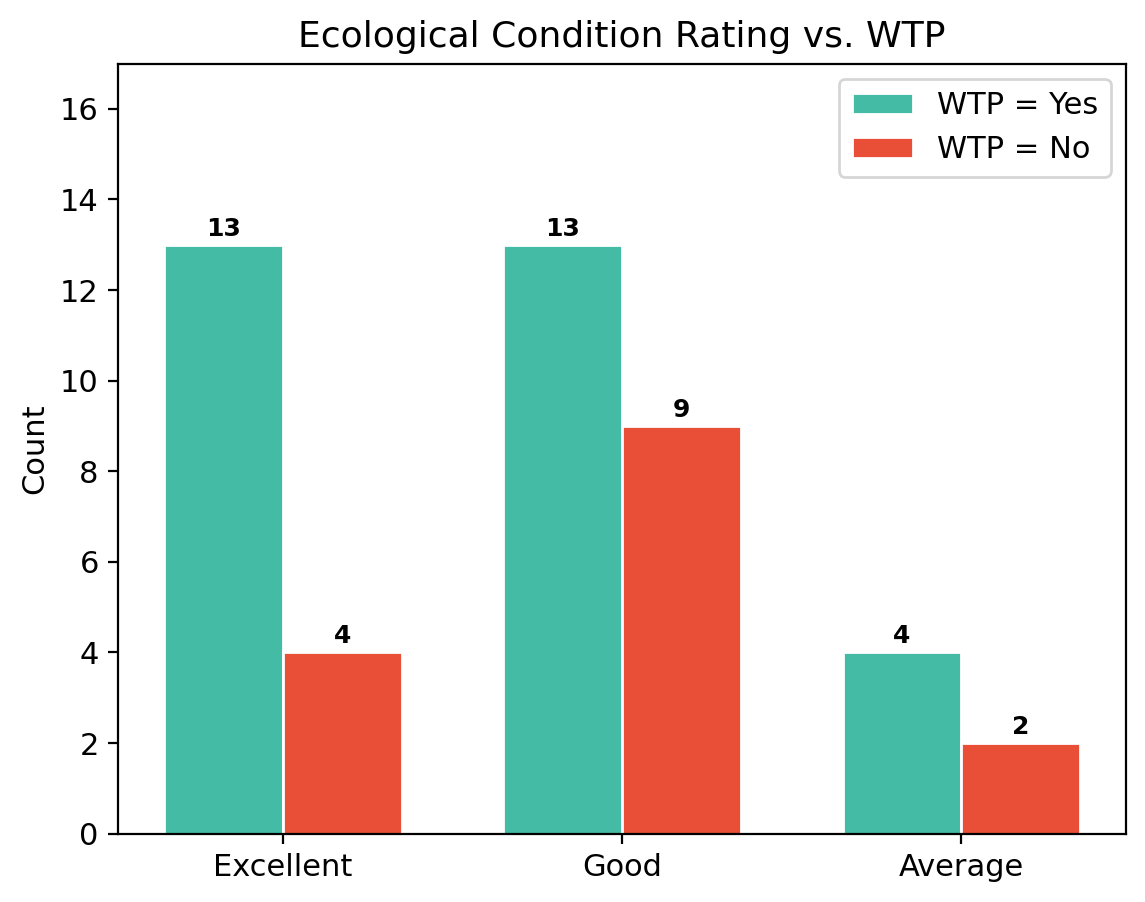
\includegraphics[width=0.6\textwidth]{figures/22_eco_vs_wtp.png}
    \caption{Ecological condition rating vs.\ WTP.}
    \label{fig:eco_wtp}
\end{figure}

% ════════════════════════════════════════════════════════════
%  6.  TOTAL ECONOMIC VALUE
% ════════════════════════════════════════════════════════════
\section{Total Economic Value Estimation}

Combining the CVM and TCM results, we estimate the Total Economic Value of Sunder Nursery as follows:

\begin{table}[H]
\centering
\caption{Total Economic Value breakdown for Sunder Nursery.}
\label{tab:tev}
\begin{tabular}{llr}
\toprule
\textbf{Component} & \textbf{Method} & \textbf{Value (\rupee\,crore/year)} \\
\midrule
Use Value (Consumer Surplus)           & TCM & 21.35 \\
Direct WTP for Conservation            & CVM & 4.00 \\
Non-Use Value (Bequest + Existence)    & CVM $\times$ 0.59 & 2.36 \\
\midrule
\textbf{Total Economic Value}          &     & \textbf{27.71} \\
\bottomrule
\end{tabular}
\end{table}

The non-use scaling factor was derived from the survey responses: 68.9\% rated future preservation as ``very important'' (bequest component) and 82.2\% would support conservation without ever visiting again (existence component). The total CVM multiplier is computed as:

\begin{equation}
    \text{Total multiplier} = 1 + (0.689 \times 0.5) + (0.822 \times 0.3) = 1.59
\end{equation}

The non-use component is then $(1.59 - 1) = 0.59$ times the direct CVM WTP, i.e.\ \rupee 4.00 $\times$ 0.59 = \rupee 2.36 crore per year.

\begin{figure}[H]
    \centering
    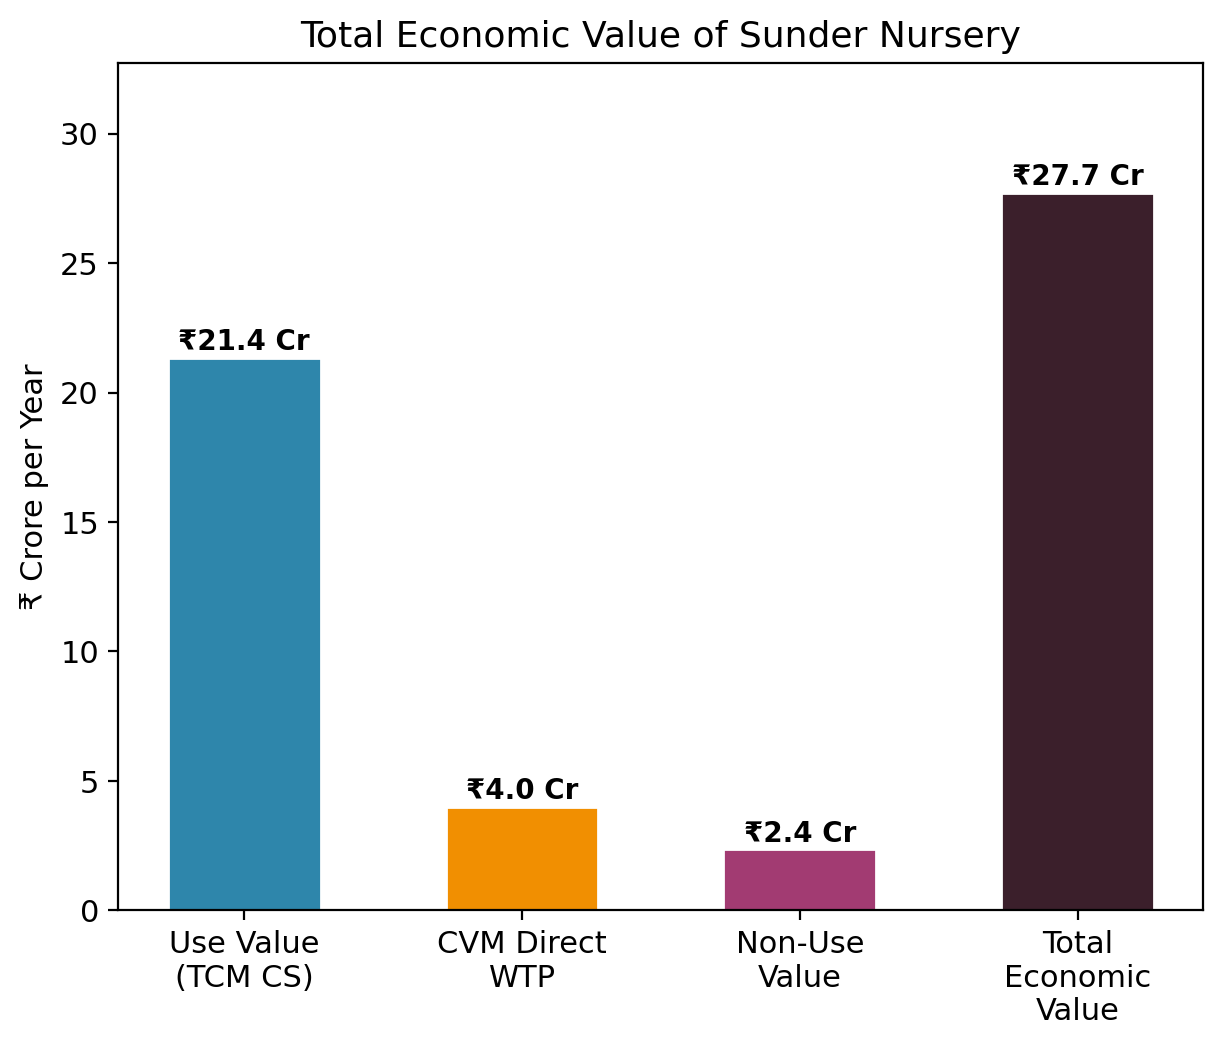
\includegraphics[width=0.65\textwidth]{figures/21_total_economic_value.png}
    \caption{Total Economic Value breakdown of Sunder Nursery.}
    \label{fig:tev}
\end{figure}

% ════════════════════════════════════════════════════════════
%  7.  DISCUSSION
% ════════════════════════════════════════════════════════════
\section{Discussion}

\subsection{Comparison with Literature}

Our results align well with comparable studies discussed in the course ebook [7]:

\begin{itemize}
    \item \textbf{Lumpinee Park, Bangkok} [1]: Using the travel cost method on 187 visitors from 17 districts, the study estimated an annual consumer surplus of \$660,230. When existence value was explicitly accounted for, the capitalized value of the park jumped from \$6.6 million to \$58 million-nearly a 9$\times$ increase. Our non-use multiplier of 1.59$\times$ is more conservative, partly because our survey questions capture only a portion of the full non-use spectrum.

    \item \textbf{Colorado Wilderness} [4]: A mail survey of 218 households found that non-use (preservation) values represented 37\% of total value even at the lower end. In our study, the CVM-derived non-use value (\rupee 2.36 crore) constitutes about 8.5\% of the total, which is reasonable given that our TCM-based use value is quite large.

    \item \textbf{Kalamazoo Nature Center} [7]: The CVM survey design we followed closely mirrors the Kalamazoo questionnaire-asking what aspects respondents value, their willingness to pay through a familiar payment vehicle, and probing bequest and existence motivations.
\end{itemize}

\subsection{Ecological Evaluation}

The ecological condition ratings from our survey paint a positive picture: 86.7\% of visitors rate the condition as ``Good'' or ``Excellent,'' validating the AKTC restoration program. This is a key finding for the park's management-it confirms that the ecological improvements are visible to and appreciated by the public.

The aspects-valued data further supports this: nearly half of all respondents (46.7\%) selected ``Protection of native plants and birds'' as something they value, indicating that the biodiversity component is not just background scenery but a consciously recognized element of the park's appeal.

\subsection{Policy Implications}

\begin{enumerate}
    \item \textbf{Entry fee revision:} The current entry fee of \rupee 20-30 captures a tiny fraction of the park's true economic value (\rupee 27.71 crore annually). A modest increase of \rupee 20-50 would be acceptable to a majority of visitors (as shown by our WTP data) and could generate \rupee 3-7.5 crore in additional annual revenue for conservation.

    \item \textbf{Public investment case:} The strong ``government should pay'' sentiment among protest bidders (33\%) suggests that visitors also expect public funding for conservation. This supports the case for continued government and trust-fund investment alongside user fees.

    \item \textbf{Targeted engagement:} The high WTP among younger visitors and students suggests that educational and outreach programs (bird walks, nature trails, heritage tours) could further strengthen the conservation constituency.
\end{enumerate}

\subsection{Limitations and Potential Biases}

Following the CVM bias framework discussed in the ebook [7], we acknowledge several limitations:

\begin{enumerate}
    \item \textbf{Strategic bias:} Some respondents may have understated their WTP (free-rider behavior) or overstated it (``warm glow'' of appearing environmentally conscious) [5].
    \item \textbf{Hypothetical bias:} No real money changed hands during the survey; actual WTP when confronted with a real fee increase might differ from stated WTP.
    \item \textbf{Information bias:} The level of information provided about conservation costs and the park's ecological significance was necessarily limited in a 2-minute survey.
    \item \textbf{Sample bias:} Our survey was conducted on a single Friday evening; weekday visitors, morning joggers, and seasonal tourists may have different profiles and preferences.
    \item \textbf{Small sample size:} With 45 respondents, statistical precision is limited. Larger surveys (200+ respondents) would be needed for robust policy recommendations.
\end{enumerate}

% ════════════════════════════════════════════════════════════
%  8.  CONCLUSION
% ════════════════════════════════════════════════════════════
\section{Conclusion}

This study estimated the Total Economic Value of Sunder Nursery at approximately \textbf{\rupee 27.71 crore per year} using a combination of the Contingent Valuation Method and the Travel Cost Method. The key findings are:

\begin{enumerate}
    \item \textbf{Strong willingness to pay:} 66.7\% of visitors are willing to pay a higher entry fee for conservation, with a mean WTP of \rupee 40 per visit among willing respondents.

    \item \textbf{Robust non-use values:} 68.9\% consider preservation for future generations ``very important'' (bequest value), and 82.2\% would support conservation even without ever visiting again (existence value). These non-use values are precisely the kind of benefits that market prices fail to capture and that CVM is designed to reveal.

    \item \textbf{Ecological success:} 86.7\% of visitors rate the park's ecological condition as ``Good'' or ``Excellent,'' confirming that the decade-long Aga Khan Trust restoration has achieved its ecological goals.

    \item \textbf{Significant consumer surplus:} The TCM analysis reveals a consumer surplus of \rupee 142 per visitor, translating to approximately \rupee 21.35 crore annually-far exceeding the revenue generated by the nominal entry fee.
\end{enumerate}

Sunder Nursery is more than a park; it is a living demonstration of how heritage conservation and ecological restoration can create lasting public value. Our analysis shows that this value, while largely invisible to the market, is very much perceived and cherished by the people who visit it-and even by those who simply want to know it exists.

\begin{figure}[H]
    \centering
    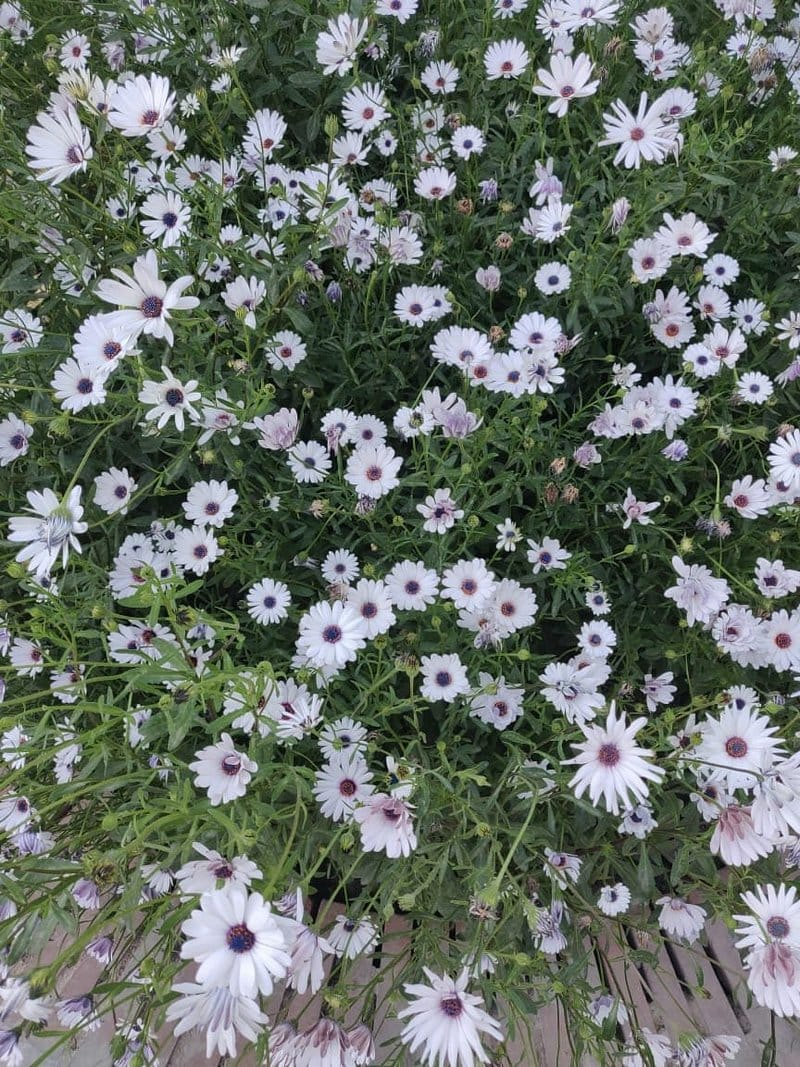
\includegraphics[width=0.7\textwidth]{../Images/12.jpeg}
    \caption{White daisies at Sunder Nursery-a symbol of the park's flourishing ecological condition.}
    \label{fig:closing}
\end{figure}

% ════════════════════════════════════════════════════════════
%  REFERENCES
% ════════════════════════════════════════════════════════════
\section*{References}
\addcontentsline{toc}{section}{References}

\begin{enumerate}[label={[\arabic*]}, nosep]
    \item Dixon, J.A.\ and Hufschmidt, M.M.\ (1986). \textit{Economic Valuation Techniques for the Environment: A Case Study Workbook}. Johns Hopkins University Press.
    \item Krutilla, J.V.\ (1967). Conservation reconsidered. \textit{American Economic Review}, 57(4), 777-786.
    \item Johansson, P.O.\ (1990). \textit{The Economic Theory and Measurement of Environmental Benefits}. Cambridge University Press.
    \item Walsh, R.G., Loomis, J.B., and Gillman, R.A.\ (1984). Valuing option, existence, and bequest demands for wilderness. \textit{Land Economics}, 60(1), 14-29.
    \item Schulze, W.D., d'Arge, R.C., and Brookshire, D.S.\ (1981). Valuing environmental commodities. \textit{Western Journal of Agricultural Economics}, 6(2), 11-22.
    \item Aga Khan Trust for Culture (2018). \textit{Sunder Nursery Heritage Park: Conservation and Landscape Restoration}. New Delhi.
    \item RDL725 Course Material: \textit{Valuing the Environment-Environmental Evaluation Techniques} (Prof.\ Vivek Kumar, IIT Delhi).
\end{enumerate}

\end{document}
